\documentclass[11pt]{article}
\usepackage[utf8]{inputenc}
\usepackage[T1]{fontenc}
\usepackage{amsmath,amssymb,amsthm}
\usepackage{graphicx}
\usepackage{booktabs}
\usepackage{array}
\usepackage[margin=2.4cm]{geometry}
\usepackage{hyperref}
\emergencystretch=2em

% The figures are written by scripts/connes_stormer_figures.py into figures/; the generated numbers live in
% ../article/generated (written by scripts/connes_stormer.py). The arXiv archive (scripts/make_arxiv_connes_stormer.sh)
% copies both next to this file.
\graphicspath{{figures/}}
\IfFileExists{generated/connes_stormer.tex}{\input{generated/connes_stormer.tex}}{%
  % generated by scripts/*.py -- do not edit by hand
\newcommand{\CSDevice}{CPU (4 threads)}
\newcommand{\CSMode}{full}
\newcommand{\CSTorch}{2.14.1+cu130}
\newcommand{\CSCuda}{none}
\newcommand{\CSCusolver}{none}
\newcommand{\CSMatmul}{FP32}
\newcommand{\CSTwoRows}{%
0.99 & 0.056002 & 0.132043 & 0.132043 & -0.2438 & 0.132771 \\
0.95 & 0.198515 & 0.290618 & 0.290618 & -0.1864 & 0.298915 \\
0.9 & 0.325083 & 0.402396 & 0.402396 & -0.1452 & 0.426476 \\
0.8 & 0.500402 & 0.542607 & 0.542607 & -0.0899 & 0.614559 \\
0.7 & 0.610864 & 0.627949 & 0.627949 & -0.0504 & 0.768305 \\
0.6 & 0.673012 & 0.676658 & 0.676658 & -0.0205 & 0.907586 \\
0.5 & 0.693147 & 0.693147 & 0.693147 & +0.0000 & 1.041035 \\
}
\newcommand{\CSTwoDevLib}{5\times10^{-13}}
\newcommand{\CSTwoDevNumpy}{4\times10^{-16}}
\newcommand{\CSTwoStarts}{16}
\newcommand{\CSKappa}{1.3255}
\newcommand{\CSRows}{%
3 & 300 & 8/8 & 22 & $7\times10^{-3}$ & $8\times10^{-12}$ & 0.0002 & 0.0322 & 0.1333 & 300 \\
4 & 150 & 8/8 & 6 & $3\times10^{-4}$ & $1\times10^{-11}$ & 0.0047 & 0.0327 & 0.1762 & 150 \\
5 & 24 & 16/16 & 2 & $5\times10^{-4}$ & $7\times10^{-13}$ & 0.0122 & 0.0323 & 0.0849 & 24 \\
}
\newcommand{\CSSteps}{1200}
\newcommand{\CSFiveSteps}{2000}
\newcommand{\CSExtStarts}{64}
\newcommand{\CSFlag}{1\times10^{-8}}
\newcommand{\CSDigits}{50}
\newcommand{\CSThreeU}{300}
\newcommand{\CSThreeFlagged}{22}
\newcommand{\CSThreeAgree}{8\times10^{-12}}
\newcommand{\CSThreeDirs}{4}
\newcommand{\CSThreeNaiveMin}{0.004}
\newcommand{\CSThreeStressStarts}{1024}
\newcommand{\CSThreeGapMax}{6.9\times10^{-3}}
\newcommand{\CSThreeGapMin}{3\times10^{-7}}
\newcommand{\CSThreeGeneral}{0.5727784466}
\newcommand{\CSThreeBasis}{0.5659197506}
\newcommand{\CSThreeOverlap}{0.897}
\newcommand{\CSThreeResidual}{1\times10^{-50}}
\newcommand{\CSFourU}{150}
\newcommand{\CSFourFlagged}{6}
\newcommand{\CSFourAgree}{1\times10^{-11}}
\newcommand{\CSFourDirs}{5}
\newcommand{\CSFourNaiveMin}{0.026}
\newcommand{\CSFourStressStarts}{1024}
\newcommand{\CSFourGapMax}{2.5\times10^{-4}}
\newcommand{\CSFourGapMin}{1\times10^{-5}}
\newcommand{\CSFourGeneral}{1.0949192541}
\newcommand{\CSFourBasis}{1.0946676581}
\newcommand{\CSFourOverlap}{0.980}
\newcommand{\CSFourResidual}{3\times10^{-50}}
\newcommand{\CSFiveU}{24}
\newcommand{\CSFiveFlagged}{2}
\newcommand{\CSFiveAgree}{7\times10^{-13}}
\newcommand{\CSFiveDirs}{6}
\newcommand{\CSFiveNaiveMin}{0.076}
\newcommand{\CSFiveStressStarts}{1024}
\newcommand{\CSFiveGapMax}{5.3\times10^{-4}}
\newcommand{\CSFiveGapMin}{1\times10^{-6}}
\newcommand{\CSFiveGeneral}{1.1963669266}
\newcommand{\CSFiveBasis}{1.1958404880}
\newcommand{\CSFiveOverlap}{0.991}
\newcommand{\CSFiveResidual}{2\times10^{-50}}
\newcommand{\CSSelf}{1\times10^{-17}}
\newcommand{\CSFourierDev}{1\times10^{-10}}
\newcommand{\CSNonabA}{0.6319, 0.5142}
\newcommand{\CSNonabASpread}{1\times10^{-13}}
\newcommand{\CSNonabAG}{0.6931, 0.6931}
\newcommand{\CSNonabB}{0.6795, 0.6923}
\newcommand{\CSNonabBSpread}{3\times10^{-6}}
\newcommand{\CSNonabBG}{0.6931, 0.6931}
\newcommand{\CSSeconds}{688}
}

\DeclareMathOperator{\Tr}{Tr}
\DeclareMathOperator{\Ad}{Ad}
\DeclareMathOperator{\artanh}{artanh}
\DeclareMathOperator{\conv}{conv}
\DeclareMathOperator{\diag}{diag}
\newcommand{\C}{\mathbb{C}}
\newcommand{\R}{\mathbb{R}}
\newcommand{\Z}{\mathbb{Z}}
\newcommand{\M}{\mathcal{M}}
\newcommand{\D}{\mathcal{D}}
\theoremstyle{plain}
\newtheorem{theorem}{Theorem}[section]
\newtheorem{proposition}[theorem]{Proposition}
\newtheorem{lemma}[theorem]{Lemma}
\newtheorem{corollary}[theorem]{Corollary}
\newtheorem*{thmA}{Theorem A}
\newtheorem*{thmB}{Theorem B}
\theoremstyle{definition}
\newtheorem{definition}[theorem]{Definition}
\newtheorem{conjecture}[theorem]{Conjecture}
\newtheorem{observation}[theorem]{Observation}
\theoremstyle{remark}
\newtheorem{remark}[theorem]{Remark}

\title{The Connes--St{\o}rmer entropy of two maximal abelian\\ subalgebras of $M_2$: an explicit variational formula,\\
and partitions that beat bases in $M_n$}
\author{Irina Nikolaeva \and Andrej Novikov}
\date{}

\begin{document}
\maketitle

\begin{abstract}
The Connes--St{\o}rmer relative entropy $H(P|Q)$ measures the relative position of two subalgebras $P,Q$ of a finite
von Neumann algebra. For the diagonal masa $\Delta_n$ of $M_n(\C)$ and a rotated copy $U\Delta_nU^*$, Choda's value
$h(U)$, the averaged row entropy of the unistochastic matrix $(|u_{ij}|^2)$, is a lower bound; Petz, Sz\'ant\'o and
Weiner showed that it is not the entropy already for $n=2$, and a formula has remained open even in that case. We prove
that for $U\in U(2)$ with $|u_{11}|^2=\cos^2\theta$ the entropy is the largest integral of
$\psi(\beta)=\sin2\beta\log\tan^2\beta$ over a window of length $\theta$, and that it is attained by an orthonormal basis
from the one-parameter family used by Petz, Sz\'ant\'o and Weiner, whose angle we locate. The mechanism is the antipodal
symmetry of the Bloch ball, which forces the entropy to equal the maximum of an entropy difference over single states.
Consequently $H=\kappa\theta+O(\theta^3)$ with $\kappa=\max\psi\approx\CSKappa$, whereas $h(U)\sim2\theta^2\log\frac1\theta$.
For $n\ge3$ the symmetry is lost. We give a first-order criterion under which Choda's partition is not optimal, valid on
an open set of unitaries in every dimension, and a numerical study for $n=3,4,5$: for a small fraction of Haar-random
$U$ the best partitions found have $n+1$ rank-one elements and beat every orthonormal basis found.
\end{abstract}

\noindent\textbf{Keywords:} Connes--St{\o}rmer entropy; relative position of subalgebras; maximal abelian subalgebras;
unistochastic matrices; mutually unbiased bases; entropic uncertainty; partitions of unity.\\
\textbf{MSC 2020:} 46L37, 94A17; 46L55, 15B51, 81P45.

\section{Introduction}\label{sec:intro}

\subsection{The relative position of two subalgebras}

A pair of subspaces of a finite-dimensional Hilbert space is determined up to unitary equivalence by their dimensions and
the principal angles between them. For two subalgebras of a von Neumann algebra no such complete invariant is available, and a number of numerical invariants have
been proposed to measure how far the two algebras are from each other: the Jones index and the Pimsner--Popa
probabilistic index for inclusions~\cite{jones1983,pimsner1986}, Popa's notion of orthogonal pairs~\cite{popa1983},
angles and distances between subalgebras (see the recent work of Bakshi and Guin~\cite{bakshi} and of Ghosh and
Kumar~\cite{ghosh2026}), and the relative entropy of Connes and St{\o}rmer~\cite{connes1975}, the subject of this paper.

Let $\M$ be a finite von Neumann algebra with a faithful normal tracial state $\tau$, let $\eta(t)=-t\log t$, and for a
von Neumann subalgebra $P\subset\M$ let $E_P$ denote the $\tau$-preserving conditional expectation onto $P$. The
Connes--St{\o}rmer relative entropy of two subalgebras $P,Q$ is
\begin{equation}\label{eq:cs}
  H(P|Q)=\sup\sum_j\bigl[\tau\eta(E_Qx_j)-\tau\eta(E_Px_j)\bigr],
\end{equation}
the supremum being taken over all finite partitions of unity $x_j\ge0$, $\sum_jx_j=1$, in $\M$. Each term compares how
much a positive element $x_j$ is ``smeared out'' by the two conditional expectations: if $x_j$ lies in $P$, then
$E_Px_j=x_j$ while $E_Qx_j$ may be much more mixed. The trivial partition $x_1=1$ shows $H(P|Q)\ge0$, and $H(P|P)=0$. If
$P\subset Q$, every term is non-positive by the concavity of $\eta$, so $H(P|Q)=0$; $H(P|Q)$ is therefore a measure of the
part of $P$ that is not contained in $Q$. Connes and St{\o}rmer introduced~\eqref{eq:cs} for finite-dimensional
subalgebras as the basic ingredient of their entropy of automorphisms~\cite{connes1975}; Pimsner and Popa extended it to
arbitrary subalgebras and related the entropy $H(\M|N)$ of an inclusion of type~II$_1$ factors to the Jones index and to
their probabilistic index~\cite{pimsner1986,jones1983}.

\subsection{Two maximal abelian subalgebras}

The simplest pair of subalgebras for which~\eqref{eq:cs} is not trivial is a pair of maximal abelian subalgebras (masas)
of $M_n=M_n(\C)$ with $\tau=\Tr/n$: the diagonal algebra $\Delta_n$ and a rotated copy $U\Delta_nU^*$, $U$ unitary. In
the language of quantum mechanics these are two non-degenerate observables, or two orthonormal bases of $\C^n$: the
standard basis and the columns of $U$. Choosing the partition into the minimal projections $e_{jj}$ of $\Delta_n$ gives
the lower bound
\begin{equation}\label{eq:choda}
  H(\Delta_n|U\Delta_nU^*)\ \ge\ h(U)=\frac1n\sum_{i,j}\eta\bigl(|u_{ij}|^2\bigr),
\end{equation}
the Shannon entropy of the rows of the unistochastic matrix $(|u_{ij}|^2)$, averaged over the rows. Choda~\cite{choda}
showed that $h(U)$ is the value of a modified relative entropy in which the partitions are restricted to $\Delta_n$, and it
was expected that $h(U)$ is also the value of $H$. At one extreme this is correct: if the two masas are complementary
(equivalently, $|u_{ij}|^2=\frac1n$ for all $i,j$, i.e.\ $\sqrt n\,U$ is a complex Hadamard matrix and the two bases are
mutually unbiased), then $h(U)=\log n$, which is the largest possible value of $H$, and Petz, Sz\'ant\'o and Weiner proved that
$H=\log n$ holds only for complementary masas~\cite[Theorem~3]{petz2009}. Away from this extreme, however, they showed that
already for $n=2$ the inequality~\eqref{eq:choda} is strict in general, and remarked that the correction of the formula
``seems to be a hard problem''~\cite[Appendix]{petz2009}. Bakshi and Guin, who need lower bounds for the entropy of pairs
of spin model subfactors built from $2\times2$ complex Hadamard matrices, use $h(U)$ and note that a formula for
$H(\Delta_n|U\Delta_nU^*)$ is open even for $n=2$~\cite[Section~2.3 and Theorem~6.22]{bakshi}.

What makes the problem hard is the nature of the supremum in~\eqref{eq:cs}. It is taken over partitions of arbitrary
length whose elements need not commute with each other or with either algebra, and the functional is neither convex nor
concave in the partition. Petz, Sz\'ant\'o and Weiner rewrote it as a maximisation over ensembles of states with
barycentre $\frac1n$ (Proposition~\ref{prop:psw}): with
\[
  G(\rho)=S(E_Q\rho)-S(E_P\rho)
\]
for a density matrix $\rho$ and the von Neumann entropy $S$, $H(P|Q)$ is the largest average of $G$ over ensembles
$\{t_j,\rho_j\}$ with $\sum_jt_j\rho_j=\frac1n$. Geometrically, $H(P|Q)$ is the value at the centre $\frac1n$ of the concave
envelope of $G$ on the state space, and in particular $H(P|Q)\le G^*:=\max G$ (Proposition~\ref{prop:envelope}).

\subsection{Results for \texorpdfstring{$n=2$}{n=2}: why the qubit case is solvable}

For $n=2$ the state space is the Bloch ball, and the observation that unlocks the problem is that the antipodal map
$r\mapsto-r$, i.e.\ $\rho\mapsto1-\rho$, preserves $G$ for every pair of subalgebras of $M_2$: a $2\times2$ density matrix
and its reflection have the same spectrum up to order, and conditional expectations are unital. A maximiser $\rho^*$ of
$G$ and its antipode $1-\rho^*$ average to $\frac12$, so the concave envelope at the centre is just the maximum,
$H=G^*$, and an optimal partition is $\{\rho^*,1-\rho^*\}$ (Lemma~\ref{lem:antipodal}). For two masas we show further
that $G$ is maximised at a pure state in the great circle spanned by the Bloch vectors of the two bases, so the optimum is
an orthonormal basis, and the maximisation over that circle reduces to a one-dimensional problem. To state the result,
write $h_2(p)=\eta(p)+\eta(1-p)$ for the binary entropy and
\begin{equation}\label{eq:psi}
  \psi(\beta)=\sin(2\beta)\log\tan^2\beta\qquad(\beta\in\R),
\end{equation}
extended by continuity with $\psi=0$ on $\frac\pi2\Z$. Every unitary $U\in M_2$ satisfies $|u_{11}|=|u_{22}|=\cos\theta$ for
a unique $\theta\in[0,\frac\pi2]$, the angle between the lines $\C e_1$ and $\C Ue_1$; Choda's value is $h(U)=h_2(\cos^2\theta)$.

\begin{thmA}
Let $U\in M_2$ be unitary, $c=|u_{11}|^2=\cos^2\theta$ with $\theta\in[0,\frac\pi2]$, and
\[
  \varphi(\alpha)=h_2\bigl(\cos^2(\alpha-\theta)\bigr)-h_2(\cos^2\alpha)=\int_{\alpha-\theta}^{\alpha}\psi(\beta)\,d\beta .
\]
Then $H(\Delta_2|U\Delta_2U^*)=\max_{\alpha\in\R}\varphi(\alpha)=G^*$. The maximum is attained by the partition into the two
projections onto an explicit orthonormal basis of $\C^2$, determined by a maximiser $\alpha^*$ of $\varphi$ and the phases
of $U$. For $\frac12<c<1$ the maximiser is unique modulo $\frac\pi2$, lies in $(\theta-\frac\pi4,0)$ and is the unique
solution there of $\psi(\alpha)=\psi(\alpha-\theta)$; $H$ is invariant under $c\mapsto1-c$
(Theorem~\ref{thm:n2} and Proposition~\ref{prop:angle}).
\end{thmA}

Thus $\varphi(\alpha)$ is the value of the basis at angle $\alpha$, and it is the area under $\psi$ over the window
$[\alpha-\theta,\alpha]$. Choda's partition is the window $[-\theta,0]$; the optimal basis slides the window so that it
captures the hump of $\psi$ on $(-\frac\pi4,0)$ (Figure~\ref{fig:window}). The optimal basis lies on the other side of
the standard basis than the basis of $U\Delta_2U^*$ (Figure~\ref{fig:bloch}): it gives up some entropy of $E_{\Delta_2}x_j$
in exchange for more entropy of $E_{U\Delta_2U^*}x_j$. Integrating $\psi\le\kappa:=\max\psi$ over the window gives a bound
linear in the angle, and a Taylor expansion at the maximum of $\psi$ shows that it is sharp to first order.

\begin{thmB}
With the notation of Theorem~A, $h(U)\le H(\Delta_2|U\Delta_2U^*)\le\kappa\min(\theta,\frac\pi2-\theta)$, where
$\kappa=2\sqrt{1-y^2}/y\approx\CSKappa$ and $y\in(0,1)$ is the unique solution of $y\artanh y=1$. As $\theta\to0$,
\[
  H(\Delta_2|U\Delta_2U^*)=\kappa\theta-\frac{\kappa+4/\kappa}{6}\,\theta^3+O(\theta^4),\qquad
  h(U)=2\theta^2\log\frac1\theta+\theta^2+O\Bigl(\theta^4\log\frac1\theta\Bigr)
\]
(Theorem~\ref{thm:bound}).
\end{thmB}

The qualitative message is that for two nearby masas the Connes--St{\o}rmer entropy is of \emph{first} order in the angle
between them, while Choda's value is of second order up to a logarithm; in particular $H/h(U)\to\infty$ as $\theta\to0$.
Restricting the partitions to one of the two algebras, as in Choda's modified entropy, loses the leading-order term
entirely (Figure~\ref{fig:asym}).

\paragraph{Relation to the work of Petz, Sz\'ant\'o and Weiner.} In the appendix of~\cite{petz2009} the authors consider,
for $\Delta_2$ and the masa generated by $\sin\beta\,\sigma_1+\cos\beta\,\sigma_3$, the one-parameter family of partitions
$\{r(t),1-r(t)\}$ with $r(t)=\frac12(1+\sin t\,\sigma_1+\cos t\,\sigma_3)$, and the resulting lower bound $f(t)\le H$; they
show that $f'(0)\ne0$ in general, so that Choda's partition $t=0$ is not optimal (Corollary~\ref{cor:choda}). In our
normal form $\beta=2\theta$ and $f(t)=\varphi(t/2)$. Theorem~A therefore says precisely that the supremum over \emph{all}
partitions is attained inside their family, $H=\max_tf(t)$. What is new is the proof that no other partition does
better, whatever the number of its elements, their ranks and the position of their Bloch vectors, and the location of
the optimal parameter; the family itself, the function $f$ and the non-optimality of $t=0$ are theirs.

\subsection{Results for \texorpdfstring{$n\ge3$}{n>=3}}

For $n\ge3$ the mechanism breaks down. The natural analogue of the antipodal map is the point reflection
$\rho\mapsto\frac2n-\rho$ through the centre of the state space, but it maps a pure state to an operator with the negative
eigenvalue $\frac2n-1$; there is no symmetry pairing maximisers of $G$ around $\frac1n$. Two things survive. First, a
first-order perturbation of Choda's partition shows $H(\Delta_n|U\Delta_nU^*)>h(U)$ whenever a certain matrix built from
$U$, $M_U=(u_{jk}\log|u_{jk}|^2)_{jk}\,U^*$, is not Hermitian (Proposition~\ref{prop:firstorder}); this holds on an open
set of unitaries in every dimension and recovers the result of Petz, Sz\'ant\'o and Weiner for $n=2$. Second, we
computed $H(\Delta_n|U\Delta_nU^*)$ numerically for Haar-random $U$ with $n=3,4,5$, maximising separately over general
partitions and over orthonormal bases (Section~\ref{sec:numerics}). The picture that emerges differs from $n=2$ in three
respects. For most unitaries the best partition found is an orthonormal basis, but for a small fraction of them (about
$7\%$ for $n=3$) the best partitions found consist of $n+1$ rank-one elements and beat every basis found, by up to
$\CSThreeGapMax$. In every sample the best value found lies strictly between $h(U)$ and the computed $G^*$, so that
neither Choda's lower bound nor the envelope bound appears to be attained. These are numerical observations: every value
we report is attained at an explicit partition and recomputed with $\CSDigits$ digits, hence it is a rigorous lower bound
for $H$ up to rounding, but the maxima over all bases are not certified. To turn the first observation into a theorem it
would suffice to certify a global upper bound for the best basis for a single unitary, a global optimisation problem over
a six-dimensional flag manifold for $n=3$; by continuity the strict inequality would then hold on a set of positive Haar
measure (Section~\ref{sec:status}).

\subsection{Related work}\label{sec:lit}

\paragraph{Entropy of subalgebras.} The relative entropy~\eqref{eq:cs} was introduced by Connes and
St{\o}rmer~\cite{connes1975} and extended to arbitrary subalgebras, with the connection to index theory, by Pimsner and
Popa~\cite{pimsner1986}; the monographs of Ohya and Petz~\cite{ohya1993} and of Neshveyev and St{\o}rmer~\cite{neshveyev2006}
treat it as part of the theory of quantum and dynamical entropy. For finite-dimensional algebras the reformulation in
terms of ensembles of states, which is our starting point, is due to Petz, Sz\'ant\'o and Weiner~\cite{petz2009}.

\paragraph{Relative position and complementarity.} Popa~\cite{popa1983} introduced orthogonal pairs of subalgebras of a
finite von Neumann algebra, $\tau(xy)=\tau(x)\tau(y)$ for $x\in P$, $y\in Q$; for masas of $M_n$ this is the complementary
case $|u_{ij}|^2=\frac1n$, and Choda showed that $h(U)=\log n$ exactly for orthogonal pairs~\cite{choda}.
Complementary subalgebras are the algebraic form of complementary observables in quantum mechanics~\cite{petz2007}; for
masas they are pairs of mutually unbiased bases~\cite{wootters1989,durt2010}, and the corresponding unitaries are rescaled
complex Hadamard matrices~\cite{tadej2006}. The matrices $(|u_{ij}|^2)$ that appear in~\eqref{eq:choda} are the unistochastic
matrices, whose geometry inside the Birkhoff polytope is intricate already for $n=3$~\cite{bengtsson2005}. Bakshi and
Guin~\cite{bakshi} compute a list of invariants of relative position (the Pimsner--Popa constant, angles, and bounds for the
Connes--St{\o}rmer entropy) for pairs of spin model subfactors, and Ghosh and Kumar~\cite{ghosh2026} relate the
Kadison--Kastler distance and the interior angle of two masas to Choda's entropy and to Popa's probabilistic index.

\paragraph{The quantum-information reading.} Let $P=\Delta_n$ and $Q=U\Delta_nU^*$. For an ensemble $\{t_j,\rho_j\}$ with
barycentre $\frac1n$, let $J$ be the label (drawn with probabilities $t_j$) and $X_P$, $X_Q$ the outcomes of measuring the
state $\rho_J$ in the standard basis and in the basis of columns of $U$. Then
\[
  \sum_jt_jG(\rho_j)=I(J:X_P)-I(J:X_Q)
\]
with the classical mutual information $I$ (Proposition~\ref{prop:info}). Hence $H(\Delta_n|U\Delta_nU^*)$ is the largest
amount by which the first measurement can be more informative than the second about the preparation of an ensemble whose
average is maximally mixed. Choda's partition, the ensemble of standard basis vectors, has $I(J:X_P)=\log n$ and
$I(J:X_Q)=\log n-h(U)$. Entropic uncertainty relations, beginning with Maassen and Uffink~\cite{maassen1988}, bound the
sum $S(E_P\rho)+S(E_Q\rho)$ from below, and averaged over an ensemble they yield Hall's information exclusion principle,
an upper bound for $I(J:X_P)+I(J:X_Q)$~\cite{hall1995}; see the review of Coles, Berta, Tomamichel and
Wehner~\cite{coles2017}. The Connes--St{\o}rmer entropy asks the complementary question about the \emph{difference} of the
two informations, under the constraint that the ensemble average is $\frac1n$.

\paragraph{What is new.} The ensemble form of $H$ (Proposition~\ref{prop:psw}), the bound $H\le\log n$, the strict
inequality $H(\Delta_2|U\Delta_2U^*)>h(U)$ for $c\notin\{0,\frac12,1\}$, the one-parameter family of bases in which our
optimum lies, and the characterisation of $H=\log n$ are due to Petz, Sz\'ant\'o and Weiner~\cite{petz2009}; the lower
bound~\eqref{eq:choda} and its interpretation are Choda's~\cite{choda}. Theorem~A, Theorem~B, the antipodal argument of
Lemma~\ref{lem:antipodal}, Proposition~\ref{prop:firstorder} and the numerical findings of Section~\ref{sec:numerics} are
new to the best of our knowledge. The envelope bound of Proposition~\ref{prop:envelope} is an elementary consequence of the
ensemble form, and Proposition~\ref{prop:info} is a direct rewriting of it; we include both because they organise the
argument and separate $n=2$ from $n\ge3$. A short account of part of these results appears as a use case in the
description of the software used for the computations~\cite{lib}.

\paragraph{Organisation.} Section~\ref{sec:prelim} collects definitions, the ensemble form and its information-theoretic
reading. Section~\ref{sec:envelope} proves the envelope bound and the antipodal lemma. Section~\ref{sec:n2} proves
Theorem~A and locates the optimal angle, and Section~\ref{sec:bounds} proves Theorem~B. Section~\ref{sec:numerics} treats
$n\ge3$: the first-order criterion, the numerical findings, and what is needed to make them rigorous.
Section~\ref{sec:open} lists open problems, and Appendix~\ref{app:numerics} describes the numerical method.

\section{Preliminaries}\label{sec:prelim}

\subsection{Conditional expectations and the entropy}

Throughout, $\M=M_n$, $\tau=\Tr/n$, and $\langle x,y\rangle_\tau=\tau(x^*y)$. Subalgebras are unital $*$-subalgebras. For such
a subalgebra $P$ the $\tau$-preserving conditional expectation $E_P$ is the orthogonal projection of $(\M,\langle\cdot,\cdot
\rangle_\tau)$ onto $P$; it is unital, positive, $P$-bimodular, preserves $\tau$ and $\Tr$, and is the unique conditional
expectation onto $P$ with these properties (see e.g.~\cite{takesaki2002}). The function $\eta(t)=-t\log t$, $\eta(0)=0$, is
continuous and concave on $[0,\infty)$; for $x\ge0$, $\eta(x)$ is defined by functional calculus, and
$S(\sigma)=\Tr\eta(\sigma)$ is the von Neumann entropy of a density matrix $\sigma$. The state space
$\D=\{\rho\in M_n:\rho\ge0,\ \Tr\rho=1\}$ is a compact convex set of real dimension $n^2-1$. We write
$h_2(p)=\eta(p)+\eta(1-p)$ for the binary entropy, $p\in[0,1]$, and reserve the letter $h$ for Choda's
value~\eqref{eq:choda}, which we regard as a function on all unitaries.

\begin{definition}\label{def:cs}
For subalgebras $P,Q\subset\M$ and $x\ge0$ put $F(x)=F_{P,Q}(x)=\tau\eta(E_Qx)-\tau\eta(E_Px)$. The Connes--St{\o}rmer relative
entropy is $H(P|Q)=\sup\sum_jF(x_j)$ over all finite families $x_1,\dots,x_m\ge0$ in $\M$ with $\sum_jx_j=1$ (partitions
of unity).
\end{definition}

\begin{lemma}\label{lem:F}
Let $P,Q\subset\M$ be subalgebras.
\begin{enumerate}
\item[(a)] $F(\lambda x)=\lambda F(x)$ for $x\ge0$ and $\lambda\ge0$. In particular, merging two elements of a partition
that are multiples of the same positive operator does not change $\sum_jF(x_j)$.
\item[(b)] Let $v\in\M$ be unitary and $\gamma=\Ad v$. Then $E_{\gamma(B)}=\gamma\circ E_B\circ\gamma^{-1}$ for every subalgebra
$B$, $F_{\gamma(P),\gamma(Q)}(\gamma(x))=F_{P,Q}(x)$, and $H(\gamma(P)|\gamma(Q))=H(P|Q)$; $\gamma$ maps optimal partitions for
$(P,Q)$ onto optimal partitions for $(\gamma(P),\gamma(Q))$.
\end{enumerate}
\end{lemma}
\begin{proof}
(a) For $s,\lambda\ge0$, $\eta(\lambda s)=\lambda\eta(s)+s\,\eta(\lambda)$, hence $\tau\eta(\lambda y)=\lambda\tau\eta(y)+\eta(\lambda)\tau(y)$
for $y\ge0$. Since $\tau(E_Qx)=\tau(E_Px)=\tau(x)$, the terms with $\eta(\lambda)$ cancel in $F(\lambda x)$. If
$x_1=a\,y$ and $x_2=b\,y$ with $a,b\ge0$, then $F(x_1)+F(x_2)=(a+b)F(y)=F(x_1+x_2)$.

(b) $\gamma$ is unitary for $\langle\cdot,\cdot\rangle_\tau$, since $\tau(\gamma(x)^*\gamma(y))=\tau(vx^*yv^*)=\tau(x^*y)$, and
$\gamma(B)$ is the image of $B$; so $\gamma E_B\gamma^{-1}$ is the orthogonal projection onto $\gamma(B)$. Moreover
$\eta(\gamma(y))=\gamma(\eta(y))$ and $\tau\circ\gamma=\tau$, so $\tau\eta(E_{\gamma(B)}\gamma(x))=\tau\gamma(\eta(E_Bx))=\tau\eta(E_Bx)$.
Since $\gamma$ maps partitions of unity bijectively onto partitions of unity, the remaining claims follow.
\end{proof}

\subsection{Two masas}

Let $\Delta_n$ be the diagonal masa and $Q_U=U\Delta_nU^*$ for a unitary $U$ with columns $u_1,\dots,u_n$. The minimal
projections of $Q_U$ are $p_k=u_ku_k^*$, and
\begin{equation}\label{eq:EQ}
  E_{\Delta_n}(x)=\sum_ke_{kk}xe_{kk},\qquad E_{Q_U}(x)=\sum_kp_kxp_k=\sum_k\langle u_k,xu_k\rangle\,p_k,
\end{equation}
since $\sum_kp_kxp_k\in Q_U$ and $\tau\bigl(p_l(x-\sum_kp_kxp_k)\bigr)=\tau(p_lx)-\tau(p_lxp_l)=0$ for every $l$. Thus the
spectrum of $E_{Q_U}x$ is the diagonal of $U^*xU$, and
\begin{equation}\label{eq:Fmasa}
  F(x)=\frac1n\Bigl[\sum_k\eta\bigl((U^*xU)_{kk}\bigr)-\sum_k\eta(x_{kk})\Bigr].
\end{equation}
The algebra $Q_U$ does not change if $U$ is multiplied from the right by a diagonal unitary or a permutation matrix, and by
Lemma~\ref{lem:F}(b) with $\gamma=\Ad D$ for a diagonal unitary $D$ (which fixes $\Delta_n$), $H(\Delta_n|Q_{DU})=H(\Delta_n|Q_U)$.
For the partition $(e_{kk})_k$, $\eta(x_{kk})\in\{\eta(0),\eta(1)\}=\{0\}$ and $(U^*e_{kk}U)_{jj}=|u_{kj}|^2$, which
gives~\eqref{eq:choda}. For an orthonormal basis $w_1,\dots,w_n$, the columns of a unitary $W$, the partition
$x_j=w_jw_j^*$ gives, by~\eqref{eq:Fmasa},
\begin{equation}\label{eq:basis}
  \sum_jF(w_jw_j^*)=h(U^*W)-h(W),
\end{equation}
and Choda's partition is the case $W=1$. We call~\eqref{eq:basis} the value of the basis $W$.

\subsection{The ensemble form}

The following reformulation is due to Petz, Sz\'ant\'o and Weiner~\cite[Section~3, Lemma~1 and (7), (8)]{petz2009}; we
include the short proof, and a Carath\'eodory argument for the attainment of the supremum.

\begin{proposition}[Petz--Sz\'ant\'o--Weiner]\label{prop:psw}
Let $P,Q\subset M_n$ be subalgebras and $G(\rho)=S(E_Q\rho)-S(E_P\rho)$ for $\rho\in\D$.
\begin{enumerate}
\item[(a)] A partition $(x_j)$ with $x_j\ne0$ corresponds to the ensemble $t_j=\tau(x_j)$, $\rho_j=x_j/\Tr x_j$, which satisfies
$t_j>0$, $\sum_jt_j=1$ and $\sum_jt_j\rho_j=\frac1n$; conversely every such ensemble defines the partition $x_j=nt_j\rho_j$.
In both directions $\sum_jF(x_j)=\sum_jt_jG(\rho_j)$.
\item[(b)] $H(P|Q)=\max\bigl\{\sum_jt_jG(\rho_j):\ t_j\ge0,\ \sum_jt_j=1,\ \sum_jt_j\rho_j=\frac1n\bigr\}$; the maximum is attained by
an ensemble of at most $n^2+1$ states. (Petz, Sz\'ant\'o and Weiner show that $n^2$ linearly independent states suffice.)
\item[(c)] $G\le\log n$ on $\D$, hence $H(P|Q)\le\log n$.
\end{enumerate}
\end{proposition}
\begin{proof}
(a) Elements $x_j=0$ contribute $F(0)=0$ and can be dropped. $\Tr x_j=n\tau(x_j)=nt_j$, so $x_j=nt_j\rho_j$, and $\sum_jx_j=1$ is
equivalent to $\sum_jt_j\rho_j=\frac1n$, which implies $\sum_jt_j=1$ by taking traces. Since $E_P\rho$ and $E_Q\rho$ are density
matrices, $F(\rho)=\frac1n[S(E_Q\rho)-S(E_P\rho)]=\frac1nG(\rho)$, and Lemma~\ref{lem:F}(a) gives $F(x_j)=nt_jF(\rho_j)=t_jG(\rho_j)$.

(b) By (a), $H$ is the supremum of $\sum_jt_jG(\rho_j)$ over finite ensembles with barycentre $\frac1n$. Identify the affine
hull of $\D$ with $\R^{n^2-1}$. For such an ensemble the point $(\frac1n,\sum_jt_jG(\rho_j))\in\R^{n^2}$ is a convex combination of
points of the graph $\{(\rho,G(\rho)):\rho\in\D\}$; by Carath\'eodory's theorem it is a convex combination of at most $n^2+1$
of them, i.e.\ there is an ensemble of at most $n^2+1$ states with the same barycentre and the same value. The ensembles of
$n^2+1$ states (zero weights allowed) with barycentre $\frac1n$ form a compact set, on which $\sum_jt_jG(\rho_j)$ is continuous,
because $S$ is continuous on $\D$ and $E_P,E_Q$ are linear. So the supremum is a maximum.

(c) $S(E_Q\rho)\le\log n$ for the density matrix $E_Q\rho$ of $M_n$, and $S(E_P\rho)\ge0$.
\end{proof}

For two masas, $G(\rho)=H_{\rm Sh}\bigl(\diag(U^*\rho U)\bigr)-H_{\rm Sh}\bigl(\diag\rho\bigr)$ with the Shannon
entropy $H_{\rm Sh}$ of a probability vector, by~\eqref{eq:EQ}.

\subsection{The information-theoretic reading}

For an ensemble $\{t_j,\rho_j\}$ and a subalgebra $P\subset M_n$ let
\[
  \chi_P\{t_j,\rho_j\}=S\Bigl(\sum_jt_jE_P\rho_j\Bigr)-\sum_jt_jS(E_P\rho_j)
\]
be the Holevo quantity of the ensemble $\{t_j,E_P\rho_j\}$, i.e.\ of the ensemble after the quantum channel $E_P$. If $P$ is
the masa of the minimal projections $p_1,\dots,p_n$, then $E_P\rho_j=\sum_k\Tr(p_k\rho_j)\,p_k$ by~\eqref{eq:EQ}, and
$\chi_P$ is the classical mutual information $I(J:X_P)$ between a label $J$ with distribution $(t_j)$ and the outcome $X_P$
of the measurement $(p_k)$ on $\rho_J$, whose conditional distribution is $\Pr(X_P=k\,|\,J=j)=\Tr(p_k\rho_j)$.

\begin{proposition}\label{prop:info}
Let $P,Q\subset M_n$ be subalgebras and $\{t_j,\rho_j\}$ an ensemble with $\sum_jt_j\rho_j=\frac1n$. Then
\[
  \sum_jt_jG(\rho_j)=\chi_P\{t_j,\rho_j\}-\chi_Q\{t_j,\rho_j\},
  \qquad\text{hence}\qquad H(P|Q)=\max\bigl(\chi_P-\chi_Q\bigr)
\]
over these ensembles. For $P=\Delta_n$ and $Q=U\Delta_nU^*$ this reads $\sum_jt_jG(\rho_j)=I(J:X_P)-I(J:X_Q)$, where $X_P$ and
$X_Q$ are the outcomes of measuring $\rho_J$ in the standard basis and in the basis $u_1,\dots,u_n$.
\end{proposition}
\begin{proof}
$E_P$ is linear and unital, so $\sum_jt_jE_P\rho_j=E_P(\frac1n)=\frac1n$ and $S(\sum_jt_jE_P\rho_j)=\log n$; the same holds for
$Q$. Hence $\chi_P-\chi_Q=\sum_jt_j\bigl[S(E_Q\rho_j)-S(E_P\rho_j)\bigr]=\sum_jt_jG(\rho_j)$, and Proposition~\ref{prop:psw}(b)
gives the formula for $H$. The last statement is the identification $\chi_P=I(J:X_P)$ above.
\end{proof}

In this language Choda's partition is the ensemble of the standard basis vectors with equal weights, for which $X_P=J$,
$I(J:X_P)=\log n$ and $I(J:X_Q)=\log n-h(U)$, and the complementary case is the one in which this ensemble is completely
invisible to the second measurement. Since the Shannon entropy of a probability vector is at least the negative logarithm
of its largest entry, $h(U)\ge-\log\max_{i,j}|u_{ij}|^2$; this is the bound of Maassen and Uffink~\cite{maassen1988} for
$S(E_P\rho)+S(E_Q\rho)$, evaluated at the basis vectors $\rho=e_{kk}$, where $S(E_P\rho)=0$.

\section{The concave envelope and the antipodal symmetry}\label{sec:envelope}

For a bounded function $g$ on $\D$ let $\hat g(\rho)=\sup\{\sum_jt_jg(\rho_j):\ \text{finite ensembles with }\sum_jt_j\rho_j=\rho\}$;
this is the smallest concave function on $\D$ that majorises $g$ (its concave envelope).

\begin{proposition}\label{prop:envelope}
Let $P,Q\subset M_n$ be subalgebras, $G$ as in Proposition~\ref{prop:psw}, $G^*=\max_\D G$ and $A=\{\rho\in\D:G(\rho)=G^*\}$.
Then
\[
  H(P|Q)=\hat G\bigl(\tfrac1n\bigr)\le G^*,
\]
and $H(P|Q)=G^*$ if and only if $\frac1n\in\conv A$. In that case the optimal partitions are exactly the partitions
$x_j=nt_j\rho_j$ with $\rho_j\in A$ whenever $t_j>0$.
\end{proposition}
\begin{proof}
The identity $H=\hat G(\frac1n)$ is Proposition~\ref{prop:psw}(b) with the definition of $\hat G$. For every ensemble,
$\sum_jt_jG(\rho_j)\le\sum_jt_jG^*=G^*$, with equality if and only if $G(\rho_j)=G^*$ whenever $t_j>0$. If $\frac1n=\sum_jt_j\rho_j$
with $\rho_j\in A$, this ensemble has the value $G^*$, so $H=G^*$. Conversely, if $H=G^*$, the maximum in
Proposition~\ref{prop:psw}(b) is attained by an ensemble with value $G^*$, all of whose states with positive weight lie in
$A$; hence $\frac1n\in\conv A$. The last statement is the equality case together with Proposition~\ref{prop:psw}(a).
\end{proof}

The bound $G^*$ is a maximisation over the $(n^2-1)$-dimensional state space, whereas $H$ requires ensembles of up to $n^2$
states with a linear constraint; any state gives a lower bound for $G^*$, any partition a lower bound for $H$. Upper bounds
for $H$ come from the dual side: if $a(\rho)=a_0+\Tr(A\rho)$ is an affine function with $a\ge G$ on $\D$, then
$\sum_jt_jG(\rho_j)\le a(\sum_jt_j\rho_j)$ for every ensemble, and so
\begin{equation}\label{eq:dual}
  H(P|Q)\le a\bigl(\tfrac1n\bigr)=a_0+\tfrac1n\Tr A .
\end{equation}
Since $\hat G$ is concave and upper semicontinuous (the maximum in Proposition~\ref{prop:psw}(b) is over a compact set),
it is the infimum of its affine majorants~\cite[Section~12]{rockafellar1970}, so these bounds are sharp in the limit. The
constant function $a=G^*$ gives Proposition~\ref{prop:envelope}.

The equality case of Proposition~\ref{prop:envelope} is exactly what a symmetry of the state space can provide.

\begin{lemma}[Antipodal symmetry]\label{lem:antipodal}
Let $n=2$ and let $P,Q\subset M_2$ be subalgebras. The map $\rho\mapsto1-\rho$ is an affine involution of $\D$ that fixes
$\frac12$ and satisfies $G(1-\rho)=G(\rho)$. Consequently $H(P|Q)=G^*$, and for every maximiser $\rho^*$ of $G$ the partition
$\{\rho^*,1-\rho^*\}$ is optimal. In the Bloch parametrisation $\rho=\frac12(1+r\cdot\sigma)$ the map is $r\mapsto-r$.
\end{lemma}
\begin{proof}
If $\rho\ge0$ and $\Tr\rho=1$, the eigenvalues $\lambda,1-\lambda\in[0,1]$ of $\rho$ give $1-\rho\ge0$, and $\Tr(1-\rho)=1$. Since
$E_P$ is linear and unital, $E_P(1-\rho)=1-E_P\rho$, and for a $2\times2$ density matrix $\sigma$ with eigenvalues $\mu,1-\mu$ the
matrix $1-\sigma$ has the eigenvalues $1-\mu,\mu$, so $S(1-\sigma)=S(\sigma)$. Hence $S(E_P(1-\rho))=S(E_P\rho)$, likewise for $Q$, and
$G(1-\rho)=G(\rho)$. If $\rho^*\in A$, then $1-\rho^*\in A$ and $\frac12=\frac12\rho^*+\frac12(1-\rho^*)\in\conv A$, so $H=G^*$ by
Proposition~\ref{prop:envelope}, with the optimal partition $x_\pm=2\cdot\frac12\rho_\pm$, $\rho_+=\rho^*$, $\rho_-=1-\rho^*$.
\end{proof}

\begin{remark}\label{rem:envelope}
(i) For $n\ge3$ the point reflection $\rho\mapsto\frac2n-\rho$ through the centre of $\D$ is affine and fixes $\frac1n$, but it
does not preserve $\D$: a pure state is mapped to an operator with the eigenvalue $\frac2n-1<0$. Nothing forces
$\frac1n\in\conv A$, and for $n=3,4,5$ the computations of Section~\ref{sec:numerics} find $G^*>H$ for every sampled unitary,
i.e.\ the optimal ensembles do not consist of maximisers of $G$.
(ii) If $U$ is complementary, $G(e_{11})=\log n=G^*$ by~\eqref{eq:Fmasa}, and $\frac1n=\frac1n\sum_ke_{kk}$ is a convex
combination of the maximisers $e_{kk}$ (all of which satisfy $G(e_{kk})=\log n$); so $H=G^*=\log n$, the partition
$(e_{kk})$ is optimal, and $h(U)=\log n$.
\end{remark}

\section{Two masas of \texorpdfstring{$M_2$}{M2}}\label{sec:n2}

\subsection{The function \texorpdfstring{$\psi$}{psi}}

Let $\Psi(\beta)=h_2(\cos^2\beta)$ and let $\psi$ be as in~\eqref{eq:psi}. Throughout, $\beta$ denotes the variable of $\psi$
and $\Psi$.

\begin{lemma}\label{lem:psi}
\begin{enumerate}
\item[(a)] $\psi$ is continuous on $\R$, odd, of period $\frac\pi2$, vanishes exactly on $\frac\pi4\Z$, and $\psi>0$ on
$(-\frac\pi4,0)$, $\psi<0$ on $(0,\frac\pi4)$.
\item[(b)] $\Psi$ is continuously differentiable on $\R$, $\Psi'=-\psi$, and $\Psi$ is even and of period $\frac\pi2$.
\item[(c)] On $(-\frac\pi4,0)$, $\psi$ has a unique critical point $\beta_\kappa$; $\psi$ is strictly increasing on
$[-\frac\pi4,\beta_\kappa]$ and strictly decreasing on $[\beta_\kappa,0]$. With $\beta_\kappa=-s^*/2$ and $y=\cos s^*$, $y\in(0,1)$ is
the unique solution of $y\artanh y=1$, and
\[
  \kappa:=\max_\R\psi=\psi(\beta_\kappa)=2\tan s^*=\frac{2\sqrt{1-y^2}}{y},\qquad \psi''(\beta_\kappa)=-4\kappa-\frac{16}\kappa .
\]
\end{enumerate}
\end{lemma}
\begin{proof}
(a) For $\beta\notin\frac\pi2\Z$, $\psi(-\beta)=-\psi(\beta)$ since $\sin$ is odd and $\tan^2$ even, and
$\psi(\beta+\frac\pi2)=\psi(\beta)$ since $\sin(2\beta+\pi)=-\sin2\beta$ and $\tan^2(\beta+\frac\pi2)=\cot^2\beta$, so that
$\log\tan^2(\beta+\frac\pi2)=-\log\tan^2\beta$. Near $0$, $|\psi(\beta)|\le2|\beta|\,|\log\tan^2\beta|\to0$, so $\psi$ is
continuous at $0$ with $\psi(0)=0$, and by periodicity at every point of $\frac\pi2\Z$. On $(0,\frac\pi4)$, $\sin2\beta>0$ and
$0<\tan^2\beta<1$, so $\psi<0$; by oddness $\psi>0$ on $(-\frac\pi4,0)$. $\psi(\pm\frac\pi4)=\pm\log1=0$. By periodicity these
are all zeros.

(b) $h_2$ is smooth on $(0,1)$ with $h_2'(p)=\log\frac{1-p}p$. For $\beta\notin\frac\pi2\Z$, $0<\cos^2\beta<1$ and
$\Psi'(\beta)=h_2'(\cos^2\beta)\cdot(-\sin2\beta)=-\sin2\beta\log\tan^2\beta=-\psi(\beta)$. At $\beta_0\in\frac\pi2\Z$, $\Psi$ is
continuous, and by the mean value theorem $(\Psi(\beta)-\Psi(\beta_0))/(\beta-\beta_0)=-\psi(\xi)$ for some $\xi$ between
$\beta_0$ and $\beta$; by continuity of $\psi$ this tends to $-\psi(\beta_0)=0$. Hence $\Psi\in C^1(\R)$, $\Psi'=-\psi$. Evenness and
periodicity follow from $\cos^2(-\beta)=\cos^2\beta$ and $h_2(\cos^2(\beta+\frac\pi2))=h_2(\sin^2\beta)=h_2(\cos^2\beta)$.

(c) Away from $\frac\pi2\Z$, $(\log\tan^2\beta)'=2/(\sin\beta\cos\beta)=4/\sin2\beta$, hence
\[
  \psi'(\beta)=2\cos2\beta\log\tan^2\beta+4,\qquad \psi''(\beta)=-4\psi(\beta)+8\cot2\beta .
\]
For $b\in(0,\frac\pi4)$ let $g(b)=\cos2b\log\tan b$, so that $\psi'(-b)=4(g(b)+1)$. Then $g'(b)=-2\sin2b\log\tan b+2\cos2b/\sin2b>0$,
$g(b)\to-\infty$ as $b\to0$ and $g(\frac\pi4)=0$. Hence $g=-1$ at exactly one point $b^*$, $\psi'>0$ on $(-\frac\pi4,-b^*)$ and
$\psi'<0$ on $(-b^*,0)$; put $\beta_\kappa=-b^*$, $s^*=2b^*\in(0,\frac\pi2)$. Since $\log\tan b=-\artanh(\cos2b)$ (both sides equal
$\frac12\log\frac{1-\cos2b}{1+\cos2b}$), the equation $g(b^*)=-1$ reads $y\artanh y=1$ with $y=\cos s^*$, and $y\artanh y$ increases
strictly from $0$ to $\infty$ on $(0,1)$. Then $\psi(\beta_\kappa)=-\sin s^*\cdot2\log\tan b^*=2\sin s^*/\cos s^*=2\tan s^*$. By (a)
the maximum of $\psi$ over a period is attained in $[-\frac\pi4,0]$, hence at $\beta_\kappa$. Finally
$\psi''(\beta_\kappa)=-4\kappa+8\cot(-s^*)=-4\kappa-8/\tan s^*=-4\kappa-16/\kappa$.
\end{proof}

\noindent Numerically $\kappa=\CSKappa$ and $\beta_\kappa\approx-0.2926$.

\subsection{The variational formula}

Write $R_\theta=\bigl(\begin{smallmatrix}\cos\theta&-\sin\theta\\ \sin\theta&\cos\theta\end{smallmatrix}\bigr)$.

\begin{lemma}\label{lem:normal}
Every unitary $U\in M_2$ can be written as $U=D_1R_\theta D_2$ with diagonal unitaries $D_1,D_2$ and $\theta\in[0,\frac\pi2]$,
$\cos^2\theta=|u_{11}|^2$. Consequently $H(\Delta_2|U\Delta_2U^*)=H(\Delta_2|R_\theta\Delta_2R_\theta^T)$, and $\gamma=\Ad D_1$ maps
optimal partitions for $R_\theta$ onto optimal partitions for $U$.
\end{lemma}
\begin{proof}
The columns and the rows of $U$ are unit vectors, so $|u_{11}|^2+|u_{21}|^2=1=|u_{11}|^2+|u_{12}|^2$ and
$|u_{12}|^2+|u_{22}|^2=1$; hence $|u_{21}|=|u_{12}|$ and $|u_{22}|=|u_{11}|$. Let $\theta\in[0,\frac\pi2]$ with $\cos\theta=|u_{11}|$
and write $u_{11}=e^{ia}\cos\theta$, $u_{21}=e^{ib}\sin\theta$, $u_{12}=-e^{ic}\sin\theta$, $u_{22}=e^{id}\cos\theta$. If
$0<\theta<\frac\pi2$, orthogonality of the columns gives $(e^{i(d-b)}-e^{i(c-a)})\cos\theta\sin\theta=0$, i.e.\
$e^{i(d-b)}=e^{i(c-a)}$, and then $U=\diag(e^{ia},e^{ib})\,R_\theta\,\diag(1,e^{i(c-a)})$, as one checks entry by
entry. If $\theta=0$, $U$ is diagonal and $U=U\cdot R_0\cdot1$; if $\theta=\frac\pi2$, $U=\diag(-u_{12},u_{21})R_{\pi/2}$.
Since $D_2\Delta_2D_2^*=\Delta_2$, $U\Delta_2U^*=\gamma(R_\theta\Delta_2R_\theta^T)$ with $\gamma=\Ad D_1$, which fixes
$\Delta_2$; Lemma~\ref{lem:F}(b) gives the rest.
\end{proof}

We use the Pauli matrices $\sigma=(\sigma_1,\sigma_2,\sigma_3)$ and the Bloch parametrisation
$\rho=\frac12(1+r\cdot\sigma)$, $r\in\R^3$, $|r|\le1$, of $\D$ for $n=2$; $\rho$ is a rank-one projection if and only if $|r|=1$. For a
unit vector $v=(\cos a,\sin a)^T$ one has $vv^*=\frac12(1+\sin2a\,\sigma_1+\cos2a\,\sigma_3)$, so its Bloch vector is
$(\sin2a,0,\cos2a)$, and the Bloch vector of $(-\sin a,\cos a)^T$ is the negative of it. Let
\[
  z=(0,0,1),\qquad q=(\sin2\theta,0,\cos2\theta),\qquad k(s)=h_2\bigl(\tfrac{1+s}2\bigr)\ (|s|\le1),
\]
so $z$ and $q$ are the Bloch vectors of $e_1$ and of $R_\theta e_1$, and $k$ is even.

\begin{lemma}\label{lem:bloch}
For $P=\Delta_2$, $Q=R_\theta\Delta_2R_\theta^T$ and $\rho=\frac12(1+r\cdot\sigma)$, $G(\rho)=f(r):=k(r\cdot q)-k(r\cdot z)$. Moreover
\begin{equation}\label{eq:series}
  k(s)=\log2-\sum_{m\ge1}\frac{s^{2m}}{2m(2m-1)}\qquad(|s|\le1),
\end{equation}
the series converging uniformly on $[-1,1]$.
\end{lemma}
\begin{proof}
$E_{\Delta_2}\rho=\diag(\rho)$ has the eigenvalues $\frac12(1\pm r_3)=\frac12(1\pm r\cdot z)$, so $S(E_{\Delta_2}\rho)=k(r\cdot z)$. By~\eqref{eq:EQ}
the eigenvalues of $E_Q\rho$ are $\langle v_1,\rho v_1\rangle$ and $\langle v_2,\rho v_2\rangle=1-\langle v_1,\rho v_1\rangle$ with
$v_1=R_\theta e_1$, and $\langle v_1,\rho v_1\rangle=\Tr(\rho v_1v_1^*)=\frac12(1+r\cdot q)$ by $\Tr\bigl((1+r\cdot\sigma)(1+q\cdot\sigma)\bigr)
=2(1+r\cdot q)$. So $S(E_Q\rho)=k(r\cdot q)$.

For~\eqref{eq:series}, $k(s)=\log2-\frac12\bigl[(1+s)\log(1+s)+(1-s)\log(1-s)\bigr]$. For $|s|<1$, integrating
$\frac{d^2}{ds^2}(1\pm s)\log(1\pm s)=1/(1\pm s)=\sum_{j\ge0}(\mp s)^j$ twice gives $(1\pm s)\log(1\pm s)=\pm s+\sum_{l\ge2}(\mp1)^ls^l/(l(l-1))$,
and adding the two expansions leaves $2\sum_{m\ge1}s^{2m}/(2m(2m-1))$. The terms are bounded by $1/(2m(2m-1))$ on $[-1,1]$, so
the series converges uniformly there (Weierstrass), its sum is continuous, and the identity extends to $s=\pm1$ by
continuity of $k$.
\end{proof}

\begin{theorem}\label{thm:n2}
Let $U\in M_2$ be unitary, $U=D_1R_\theta D_2$ as in Lemma~\ref{lem:normal}, $c=|u_{11}|^2=\cos^2\theta$, and
\[
  \varphi(\alpha)=h_2\bigl(\cos^2(\alpha-\theta)\bigr)-h_2(\cos^2\alpha)=\int_{\alpha-\theta}^{\alpha}\psi(\beta)\,d\beta .
\]
Then $\varphi$ is $C^1$ and $\frac\pi2$-periodic, $\varphi'(\alpha)=\psi(\alpha)-\psi(\alpha-\theta)$, and
\begin{enumerate}
\item[(a)] $H(\Delta_2|U\Delta_2U^*)=\max_{\alpha\in\R}\varphi(\alpha)=G^*$;
\item[(b)] for every maximiser $\alpha^*$ of $\varphi$, the projections onto the orthonormal basis $D_1(\cos\alpha^*,\sin\alpha^*)^T$,
$D_1(-\sin\alpha^*,\cos\alpha^*)^T$ form an optimal partition;
\item[(c)] $H(\Delta_2|U\Delta_2U^*)$ depends only on $c$, and it is invariant under $c\mapsto1-c$.
\end{enumerate}
\end{theorem}
\begin{proof}
By Lemma~\ref{lem:normal} we may assume $U=R_\theta$, $D_1=1$, and transport optimal partitions by $\Ad D_1$ at the end.
The integral form is $\varphi(\alpha)=\Psi(\alpha-\theta)-\Psi(\alpha)=\int_{\alpha-\theta}^\alpha\psi$ by Lemma~\ref{lem:psi}(b), which
also gives the regularity, periodicity and derivative of $\varphi$.

\emph{Step 1: $H=G^*=\max_{|r|\le1}f(r)$.} This is Lemma~\ref{lem:antipodal} together with Lemma~\ref{lem:bloch}; in the Bloch
picture, $f(-r)=f(r)$ because $k$ is even, and if $r^*$ maximises $f$, the partition $\{\rho_+,\rho_-\}$ with
$\rho_\pm=\frac12(1\pm r^*\cdot\sigma)$ is optimal.

\emph{Step 2: reduction to the unit circle in the plane of $z$ and $q$.} If $\theta\in\{0,\frac\pi2\}$, then $q=\pm z$ and $f\equiv0$
since $k$ is even; also $\varphi\equiv0$, because $h_2(\cos^2(\alpha-\frac\pi2))=h_2(\sin^2\alpha)=h_2(\cos^2\alpha)$. So $H=0=\max\varphi$
and every basis is optimal. Let $0<\theta<\frac\pi2$. Then $z$ and $q$ span the plane $\{r_2=0\}$, and $f(r)$ depends only on
the orthogonal projection $a=(r_1,0,r_3)$ of $r$ onto it, $|a|\le|r|\le1$. Write $a=\varrho(\sin\omega,0,\cos\omega)$ with
$0\le\varrho\le1$ and the polar angle $\omega$ measured from $z$; then $a\cdot z=\varrho\cos\omega$ and
$a\cdot q=\varrho\cos(\omega-2\theta)$, and by~\eqref{eq:series}
\[
  f(a)=\sum_{m\ge1}\frac{\varrho^{2m}}{2m(2m-1)}\bigl(\cos^{2m}\omega-\cos^{2m}(\omega-2\theta)\bigr).
\]
If $|\cos\omega|\ge|\cos(\omega-2\theta)|$, all terms are non-negative and non-decreasing in $\varrho$, so
$f(a)\le f(\sin\omega,0,\cos\omega)$. Otherwise all terms are non-positive and $f(a)\le0=f(\sin\theta,0,\cos\theta)$, the
value at $\omega=\theta$, where $\cos\omega=\cos(\omega-2\theta)$. Hence the maximum of $f$ over the ball equals its maximum over
the unit circle of the plane,
\[
  \max_{|r|\le1}f=\max_{\omega\in\R}\bigl[k(\cos(\omega-2\theta))-k(\cos\omega)\bigr],
\]
and it is attained at a unit vector $r^*=(\sin\omega^\circ,0,\cos\omega^\circ)$.

\emph{Step 3: the angle.} Since $k(\cos2\gamma)=h_2(\frac{1+\cos2\gamma}2)=h_2(\cos^2\gamma)$, the substitution $\omega=2\alpha$ turns
the right-hand side into $\max_\alpha\varphi(\alpha)$. This proves (a). For a maximiser $\alpha^*$ of $\varphi$, $r^*=(\sin2\alpha^*,0,
\cos2\alpha^*)$ maximises $f$, and $\rho_+$, $\rho_-$ are the projections onto $(\cos\alpha^*,\sin\alpha^*)^T$ and
$(-\sin\alpha^*,\cos\alpha^*)^T$; with Step~1 and Lemma~\ref{lem:normal} this proves (b).

(c) $\varphi$ depends only on $\theta$, i.e.\ on $c$. Let $J=\bigl(\begin{smallmatrix}0&1\\1&0\end{smallmatrix}\bigr)$. Then
$UJ\Delta_2(UJ)^*=U\Delta_2U^*$ and $|(UJ)_{11}|^2=|u_{12}|^2=1-c$.
\end{proof}

\begin{figure}[t]
\centering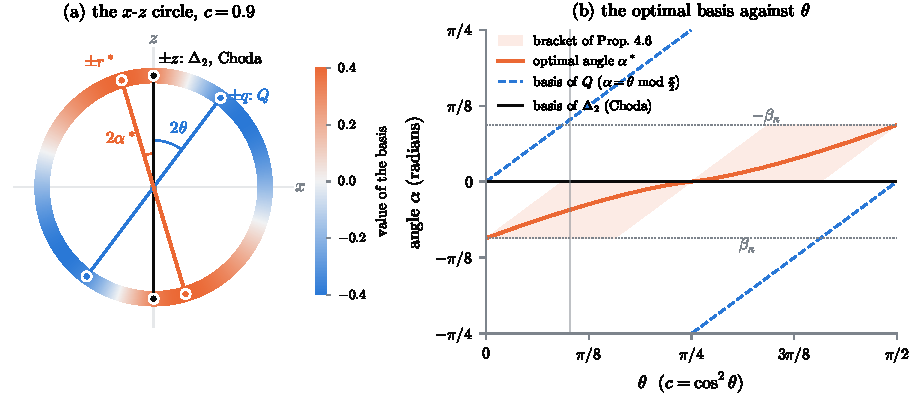
\includegraphics[width=\textwidth]{cs_bloch.pdf}
\caption{(a) The great circle $r_2=0$ of the Bloch ball for $c=0.9$ ($\theta\approx0.3218$). An orthonormal basis of $\C^2$
with real coefficients is a pair of antipodal points $\pm r$ at the polar angle $\omega=2\alpha$ from $z$, and the ring is
coloured by its value $\varphi(\alpha)$ (Theorem~\ref{thm:n2}). Black: the basis of $\Delta_2$, i.e.\ Choda's partition
(value $h(U)$); blue: the basis of $Q=U\Delta_2U^*$ (value $-h(U)$); orange: the optimal basis $\pm r^*$, at the angle
$2\alpha^*\approx-0.290$ on the other side of $z$ than $q$. (b) The optimal angle $\alpha^*\in(-\frac\pi4,\frac\pi4]$ against
$\theta$, with the bracket of Proposition~\ref{prop:angle} shaded; $\alpha^*\to\beta_\kappa$ as $\theta\to0$, $\alpha^*=0$ at
$\theta=\frac\pi4$, and $\alpha^*(\theta)=-\alpha^*(\frac\pi2-\theta)$. The thin vertical line marks $c=0.9$.}
\label{fig:bloch}
\end{figure}

\begin{remark}\label{rem:n2}
(i) At $\alpha=0$, $\varphi(0)=h_2(c)=h(U)$, the value of Choda's partition $e_{11},e_{22}$. At $\alpha=\theta$ (the basis of $Q$)
$\varphi(\theta)=-h(U)$.
(ii) In the Bloch picture (Figure~\ref{fig:bloch}), $z$ and $q$ enclose the angle $2\theta$, and the optimal Bloch vector $r^*$
has the angle $2\alpha^*$ from $z$. By Proposition~\ref{prop:angle} below, for $\frac12<c<1$ it lies on the other side of $z$
than $q$.
(iii) Let $0<c<1$. Since $H=G^*$, the optimal partitions are exactly the families $x_j=2t_j\rho_j$ with $\rho_j$ maximising
$G$ and $\sum_jt_j\rho_j=\frac12$ (Proposition~\ref{prop:envelope}). Every maximiser $r$ of $f$ has $|r|=1$ and $r_2=0$: as
$f(r)=H\ge h(U)>0$, in Step~2 of the proof we are in the case $|\cos\omega|>|\cos(\omega-2\theta)|$, where every term of the
series is strictly increasing in $\varrho$, and $r_2\ne0$ or $|r|<1$ would give $\varrho<1$. Since the maximiser of $\varphi$ is
unique modulo $\frac\pi2$ (Proposition~\ref{prop:angle}), the maximisers of $G$ are the two pure states $\rho_\pm$, and the
optimal partition is unique up to splitting $\rho_\pm$ into several multiples (Lemma~\ref{lem:F}(a)).
\end{remark}

\subsection{The optimal angle}

\begin{proposition}\label{prop:angle}
Let $\frac12<c<1$, i.e.\ $0<\theta<\frac\pi4$, and let $\beta_\kappa$ be as in Lemma~\ref{lem:psi}(c). Then $\varphi$ has a unique
maximiser $\alpha^*$ in $(-\frac\pi4,\frac\pi4]$; it satisfies
\[
  \max\bigl(\beta_\kappa,\theta-\tfrac\pi4\bigr)<\alpha^*<\min\bigl(\beta_\kappa+\theta,0\bigr),
\]
and it is the unique solution of $\psi(\alpha)=\psi(\alpha-\theta)$ in this interval. In particular $\alpha^*<0$, and
$\alpha^*\to\beta_\kappa$ as $\theta\to0$. For $0<c<\frac12$ the maximiser is $\alpha^*(c)=-\alpha^*(1-c)$. For $c=\frac12$ the
maximiser is $\alpha^*=0$ (modulo $\frac\pi2$) and $H=\log2$.
\end{proposition}
\begin{proof}
Let $I_\ell=(-\frac\pi4+\ell\frac\pi2,\ell\frac\pi2)$ and $N_\ell=(\ell\frac\pi2,\frac\pi4+\ell\frac\pi2)$, $\ell\in\Z$; by Lemma~\ref{lem:psi}(a),
$\psi>0$ on the $I_\ell$ and $\psi<0$ on the $N_\ell$, all of length $\frac\pi4$. Let $0<\theta\le\frac\pi4$ and let
$W=[\alpha-\theta,\alpha]$ be a window. If $W$ met two of the $I_\ell$, it would contain the closure of some $N_\ell$ together with
points on both sides of it, so its length would exceed $\frac\pi4$; hence $W$ meets at most one $I_\ell$, in an interval $J$ of
length at most $\theta$. Choose a window $W'\subset\overline{I_\ell}$ of length $\theta$ containing $J$. Since $\psi\ge0$ on
$\overline{I_\ell}$ and $\psi\le0$ on $W\setminus J$,
\[
  \int_W\psi\le\int_J\psi\le\int_{W'}\psi,
\]
and the first inequality is strict unless $W\setminus J$ is a null set, i.e.\ unless $W\subset\overline{I_\ell}$. Hence every
maximising window lies in some $\overline{I_\ell}$; modulo $\frac\pi2$, $W\subset[-\frac\pi4,0]$, i.e.\ $\alpha\in[\theta-\frac\pi4,0]$.

\emph{$c=\frac12$.} For $\theta=\frac\pi4$ the only such window is $[-\frac\pi4,0]$, so $\alpha^*=0$ and
$H=\Psi(-\frac\pi4)-\Psi(0)=h_2(\frac12)-h_2(1)=\log2$.

\emph{$\frac12<c<1$.} Now $0<\theta<\frac\pi4$. At the end points, $\varphi'(0)=\psi(0)-\psi(-\theta)=-\psi(-\theta)<0$ and
$\varphi'(\theta-\frac\pi4)=\psi(\theta-\frac\pi4)-\psi(-\frac\pi4)=\psi(\theta-\frac\pi4)>0$, so neither is a maximiser of the
$C^1$ function $\varphi$ on $\R$, and every maximiser $\alpha^*$ (modulo $\frac\pi2$) lies in $(\theta-\frac\pi4,0)$ and satisfies
$\varphi'(\alpha^*)=0$, i.e.\ $\psi(\alpha^*)=\psi(\alpha^*-\theta)$ with $\alpha^*-\theta<\alpha^*$ both in $(-\frac\pi4,0)$. As $\psi$ is
strictly monotone on $[-\frac\pi4,\beta_\kappa]$ and on $[\beta_\kappa,0]$ (Lemma~\ref{lem:psi}(c)), two distinct points with equal
values lie on different sides of $\beta_\kappa$: $\alpha^*-\theta<\beta_\kappa<\alpha^*$. On the interval
$L=(\max(\beta_\kappa,\theta-\frac\pi4),\min(\beta_\kappa+\theta,0))$ we have $\alpha\in(\beta_\kappa,0)$ and
$\alpha-\theta\in(-\frac\pi4,\beta_\kappa)$, so $\psi(\alpha)$ is strictly decreasing and $\psi(\alpha-\theta)$ strictly increasing
in $\alpha$; hence $\varphi'$ is strictly decreasing on $L$ and has at most one zero there. A maximiser exists by continuity and
periodicity, so it is unique modulo $\frac\pi2$. As $\theta\to0$, $L\subset(\beta_\kappa,\beta_\kappa+\theta)$ shrinks to $\beta_\kappa$.

\emph{$0<c<\frac12$.} With $\theta'=\frac\pi2-\theta$ and Lemma~\ref{lem:psi}(b),
$\varphi_\theta(\alpha)=\Psi(\alpha-\frac\pi2+\theta')-\Psi(\alpha)=\Psi(-\alpha-\theta')-\Psi(-\alpha)=\varphi_{\theta'}(-\alpha)$,
where $\varphi_\theta$ denotes $\varphi$ for the angle $\theta$; and $\cos^2\theta'=1-c$.
\end{proof}

The proof is the sliding-window picture of Figure~\ref{fig:window}: a window of length $\theta\le\frac\pi4$ that captures
the most area under $\psi$ must lie in a single positive hump of $\psi$, and within the hump it is optimal when the values of
$\psi$ at its two ends agree. As $\theta\to0$ the optimal basis therefore does not approach the basis of $\Delta_2$ (angle $0$)
or of $Q$ (angle $\theta$), but the basis at the fixed angle $\beta_\kappa$ where $\psi$ is largest (Figure~\ref{fig:bloch}(b)).

\begin{figure}[t]
\centering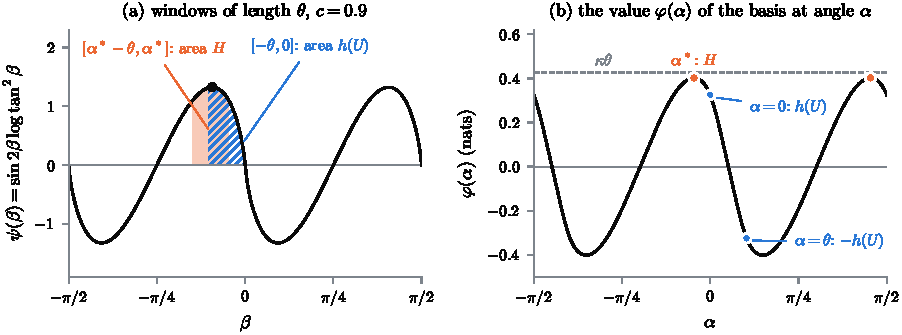
\includegraphics[width=\textwidth]{cs_window.pdf}
\caption{(a) The function $\psi$ for $c=0.9$. By Theorem~\ref{thm:n2} the value of the basis at angle $\alpha$ is the area
under $\psi$ over the window $[\alpha-\theta,\alpha]$. Choda's partition corresponds to the window $[-\theta,0]$ (hatched, area
$h(U)$); the optimal basis to the window of the same length with the largest area, which straddles the maximum
$\kappa=\psi(\beta_\kappa)$ (dot) and whose end points have equal values of $\psi$ (shaded, area $H$). (b) The value
$\varphi(\alpha)$ of the basis at angle $\alpha$, with the three bases of Figure~\ref{fig:bloch} and the upper bound
$\kappa\theta$ of Theorem~\ref{thm:bound}.}
\label{fig:window}
\end{figure}

\section{Bounds and asymptotics for \texorpdfstring{$n=2$}{n=2}}\label{sec:bounds}

\begin{theorem}\label{thm:bound}
Let $U\in M_2$ be unitary, $c=|u_{11}|^2=\cos^2\theta$, $\theta\in[0,\frac\pi2]$, and $\kappa=\max\psi$ as in
Lemma~\ref{lem:psi}(c). Then
\begin{enumerate}
\item[(a)] $h(U)=h_2(c)\le H(\Delta_2|U\Delta_2U^*)\le\kappa\min\bigl(\theta,\frac\pi2-\theta\bigr)$;
\item[(b)] as $\theta\to0$,
\[
  H(\Delta_2|U\Delta_2U^*)=\kappa\theta-\frac{\kappa+4/\kappa}6\theta^3+O(\theta^4),\qquad
  h(U)=2\theta^2\log\frac1\theta+\theta^2+O\Bigl(\theta^4\log\frac1\theta\Bigr);
\]
in particular $H/h(U)\to\infty$ as $c\to1$, and likewise as $c\to0$.
\end{enumerate}
\end{theorem}
\begin{proof}
(a) The lower bound is $\varphi(0)=h_2(c)$. For every $\alpha$, $\varphi(\alpha)=\int_{\alpha-\theta}^\alpha\psi\le\theta\max\psi=\kappa\theta$, so
$H\le\kappa\theta$ by Theorem~\ref{thm:n2}(a). Applying this to $1-c$, whose angle is $\frac\pi2-\theta$, and using
Theorem~\ref{thm:n2}(c) gives $H\le\kappa(\frac\pi2-\theta)$.

(b) Fix $\delta>0$ with $[\beta_\kappa-\delta,\beta_\kappa+\delta]\subset(-\frac\pi4,0)$; $\psi$ is smooth there, and by Taylor's theorem
there is $C$ with $|\psi(\beta)-\kappa-\frac12\psi''(\beta_\kappa)(\beta-\beta_\kappa)^2|\le C|\beta-\beta_\kappa|^3$ for
$|\beta-\beta_\kappa|\le\delta$. Let $\theta<\min(\delta,\frac\pi4)$. By Proposition~\ref{prop:angle} the maximising window
$W=[\alpha^*-\theta,\alpha^*]$ contains $\beta_\kappa$, so $W\subset[\beta_\kappa-\delta,\beta_\kappa+\delta]$. Since
$\int_W(\beta-\beta_\kappa)^2d\beta\ge\theta^3/12$ for every window of length $\theta$ (with equality for the window centred at
$\beta_\kappa$), $\psi''(\beta_\kappa)<0$ and $\int_W|\beta-\beta_\kappa|^3d\beta\le\theta^4$,
\[
  \kappa\theta+\frac{\psi''(\beta_\kappa)}{24}\theta^3-C\theta^4\ \le\ \varphi\bigl(\beta_\kappa+\tfrac\theta2\bigr)\ \le\ H\ =\ \int_W\psi\ \le\
  \kappa\theta+\frac{\psi''(\beta_\kappa)}{24}\theta^3+C\theta^4 ,
\]
and $\psi''(\beta_\kappa)/24=-(\kappa+4/\kappa)/6$ by Lemma~\ref{lem:psi}(c).

For Choda's value put $s=\sin^2\theta=1-c$, so $h(U)=\eta(s)+\eta(1-s)$. Since $-\log(1-s)=s+O(s^2)$, $\eta(1-s)=s+O(s^2)=\theta^2+O(\theta^4)$.
Since $s=\theta^2(1+O(\theta^2))$ and $\log s=2\log\theta+O(\theta^2)$, $\eta(s)=-s\log s=2\theta^2\log\frac1\theta+O(\theta^4\log\frac1\theta)$.
Adding gives the expansion of $h(U)$, and $H/h(U)\sim\kappa/(2\theta\log\frac1\theta)\to\infty$. The case $c\to0$ follows from
Theorem~\ref{thm:n2}(c) and the symmetry $h_2(c)=h_2(1-c)$.
\end{proof}

\noindent Since $\theta=\arccos\sqrt c\sim\sqrt{1-c}$, near $c=1$ the entropy behaves like $\kappa\sqrt{1-c}$, much larger than
$h(U)\sim(1-c)\log\frac1{1-c}$. The bound $\log2$ of Proposition~\ref{prop:psw}(c) is better than $\kappa\min(\theta,\frac\pi2-\theta)$
near $c=\frac12$. Figure~\ref{fig:asym} compares $H$ with $h(U)$ over the whole range and checks the two expansions of
Theorem~\ref{thm:bound}(b), and Table~\ref{tab:cs2} lists values.

\begin{figure}[t]
\centering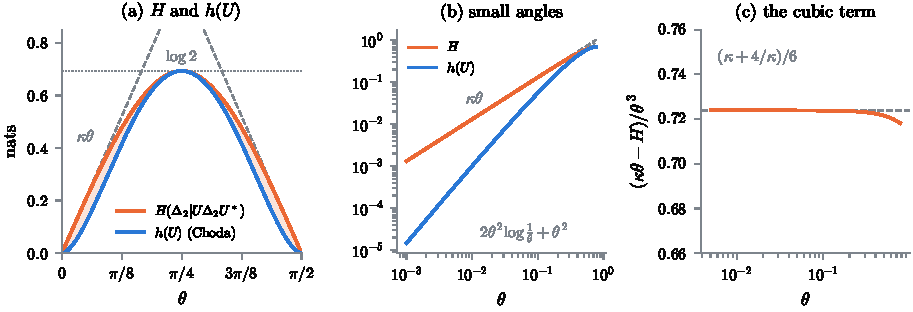
\includegraphics[width=\textwidth]{cs_asymptotics.pdf}
\caption{(a) $H(\Delta_2|U\Delta_2U^*)$ (Theorem~\ref{thm:n2}) and Choda's value $h(U)$ against $\theta$; the shaded gap
$H-h(U)$ vanishes exactly at $\theta\in\{0,\frac\pi4,\frac\pi2\}$ (Corollary~\ref{cor:choda}). Dashed: the bound
$\kappa\min(\theta,\frac\pi2-\theta)$; dotted: $\log2$. (b) The same on logarithmic axes for small $\theta$, with the leading
terms $\kappa\theta$ and $2\theta^2\log\frac1\theta+\theta^2$ of Theorem~\ref{thm:bound}(b). (c) $(\kappa\theta-H)/\theta^3$, which
tends to $(\kappa+4/\kappa)/6\approx0.724$. All curves are computed from the formulas of Section~\ref{sec:n2}.}
\label{fig:asym}
\end{figure}

\begin{corollary}[Petz--Sz\'ant\'o--Weiner]\label{cor:choda}
$H(\Delta_2|U\Delta_2U^*)>h(U)$ unless $c\in\{0,\frac12,1\}$, where $H=h(U)$.
\end{corollary}
\begin{proof}
This is~\cite[Appendix]{petz2009}; in terms of Theorem~\ref{thm:n2} it reads as follows. $h(U)=h_2(c)=\varphi(0)$ and
$\varphi'(0)=\psi(0)-\psi(-\theta)=\psi(\theta)$, which by Lemma~\ref{lem:psi}(a) vanishes exactly for $\theta\in\{0,\frac\pi4,\frac\pi2\}$.
Otherwise $0$ is not a maximiser of $\varphi$, so $H>\varphi(0)$. For $c\in\{0,1\}$, $H=0=h_2(c)$, and for $c=\frac12$,
$H=\log2=h_2(\frac12)$ (Proposition~\ref{prop:angle}).
\end{proof}

\begin{remark}[Spin model subfactors]\label{rem:bakshi}
Bakshi and Guin use the inequality $H(u\Delta_2u^*|v\Delta_2v^*)\le H(R_u|R_v)$ for the spin model subfactors $R_u,R_v$ of two
$2\times2$ complex Hadamard matrices $u,v$~\cite[proof of Theorem~6.22]{bakshi}, together with Choda's bound. By
Lemma~\ref{lem:F}(b) with $\gamma=\Ad u^*$, $H(u\Delta_2u^*|v\Delta_2v^*)=H(\Delta_2|U\Delta_2U^*)$ with $U=u^*v$, so
Theorem~\ref{thm:n2} with $c=|(u^*v)_{11}|^2$ raises their lower bound $h_2(c)$ for $H(R_u|R_v)$ to $\max_\alpha\varphi(\alpha)$,
e.g.\ from $0.3251$ to $0.4024$ at $c=0.9$ (Table~\ref{tab:cs2}).
\end{remark}

\begin{table}[t]
\centering\small
\begin{tabular}{cccccc}
\toprule
$c$ & $h(U)=h_2(c)$ & $H$, Theorem~\ref{thm:n2} & $H$, numerical search & $\alpha^*$ (radians) & $\kappa\theta$\\
\midrule
\CSTwoRows
\bottomrule
\end{tabular}
\caption[]{$H(\Delta_2|U\Delta_2U^*)$ for $c=|u_{11}|^2$: Choda's value, the variational formula of Theorem~\ref{thm:n2} with
its optimal angle $\alpha^*\in(-\frac\pi4,\frac\pi4]$, the maximum over general partitions with four elements found by the
numerical search of Appendix~\ref{app:numerics} for $U=D_1R_\theta D_2$ with random phases, and the upper bound $\kappa\theta$ of
Theorem~\ref{thm:bound}.}
\label{tab:cs2}
\end{table}

\section{Masas of \texorpdfstring{$M_n$}{Mn} for \texorpdfstring{$n\ge3$}{n>=3}}\label{sec:numerics}

\subsection{Choda's partition is generically not optimal}

For $n=2$, Corollary~\ref{cor:choda} was obtained by differentiating the value of a basis at Choda's partition. The same
first-order argument works in every dimension. For a unitary $U\in M_n$ let
\[
  A_U=\bigl(u_{jk}\log|u_{jk}|^2\bigr)_{j,k=1}^n\quad(\text{with }0\log0=0),\qquad M_U=A_UU^* .
\]
The map $U\mapsto M_U$ is continuous, since $t\mapsto t\log|t|^2$ is continuous on $\C$.

\begin{proposition}\label{prop:firstorder}
Let $U\in M_n$ be unitary, $X\in M_n$ skew-Hermitian, $W_\varepsilon=\exp(\varepsilon X)$, and let
$V(\varepsilon)=h(U^*W_\varepsilon)-h(W_\varepsilon)$ be the value~\eqref{eq:basis} of the basis $W_\varepsilon$. Then $V(0)=h(U)$
and
\[
  \lim_{\varepsilon\downarrow0}\frac{V(\varepsilon)-V(0)}{\varepsilon}=-\frac2n\,\mathrm{Re}\Tr(M_UX).
\]
Consequently, if $M_U$ is not Hermitian, then $H(\Delta_n|U\Delta_nU^*)>h(U)$; an improving direction is
$X=\frac12(M_U-M_U^*)$, for which the derivative equals $\frac2n\|X\|_2^2>0$. The set of unitaries with $M_U\ne M_U^*$ is
open, and for every $n\ge2$ it contains $R_\theta\oplus1_{n-2}$ for $\theta\notin\frac\pi4\Z$; in particular it has
positive Haar measure.
\end{proposition}
\begin{proof}
$V(0)=h(U^*)-h(1)=h(U)$, since $|(U^*)_{ij}|=|u_{ji}|$ and $h(1)=0$.

\emph{The term $h(W_\varepsilon)$ is $o(\varepsilon)$.} $W_\varepsilon=1+\varepsilon X+O(\varepsilon^2)$, so $|(W_\varepsilon)_{ij}|^2\le
C\varepsilon^2$ for $i\ne j$, and $1-|(W_\varepsilon)_{ii}|^2=\sum_{j\ne i}|(W_\varepsilon)_{ij}|^2\le C\varepsilon^2$ because the rows are unit
vectors. As $\eta(1-\delta)\le\delta$ for $\delta\in[0,1]$ and $\eta$ is increasing on $[0,e^{-1}]$, $h(W_\varepsilon)\le
C'(\varepsilon^2+\varepsilon^2\log\frac1\varepsilon)=o(\varepsilon)$ for small $\varepsilon$, and $h\ge0$.

\emph{The term $h(U^*W_\varepsilon)$.} Let $b_{ij}(\varepsilon)=(U^*W_\varepsilon)_{ij}=\overline{u_{ji}}+\varepsilon(U^*X)_{ij}+O(\varepsilon^2)$. If $u_{ji}=0$,
then $|b_{ij}|^2=O(\varepsilon^2)$ and $\eta(|b_{ij}|^2)=o(\varepsilon)$ as above. If $u_{ji}\ne0$, $\varepsilon\mapsto\eta(|b_{ij}(\varepsilon)|^2)$ is
differentiable at $0$ with derivative
$\eta'(|u_{ji}|^2)\cdot2\,\mathrm{Re}\bigl(u_{ji}(U^*X)_{ij}\bigr)=-2\bigl(1+\log|u_{ji}|^2\bigr)\mathrm{Re}\bigl(u_{ji}(U^*X)_{ij}\bigr)$.
Summing over $i,j$ (the terms with $u_{ji}=0$ may be included, as they vanish),
\begin{align*}
  \frac{d}{d\varepsilon}\Big|_{0^+}h(U^*W_\varepsilon)
  &=-\frac2n\,\mathrm{Re}\sum_{i,j}u_{ji}(U^*X)_{ij}-\frac2n\,\mathrm{Re}\sum_{i,j}(A_U)_{ji}(U^*X)_{ij}\\
  &=-\frac2n\,\mathrm{Re}\Tr(X)-\frac2n\,\mathrm{Re}\Tr(A_UU^*X).
\end{align*}
$\Tr X$ is purely imaginary, so the first term vanishes, and the second is $-\frac2n\mathrm{Re}\Tr(M_UX)$.

\emph{The improving direction.} Write $M_U=M_h+M_a$ with $M_h=\frac12(M_U+M_U^*)$ and $M_a=\frac12(M_U-M_U^*)$. For skew-Hermitian $X$,
$\Tr(M_hX)$ is purely imaginary and $\Tr(M_aX)$ is real. With $X=M_a$, $\mathrm{Re}\Tr(M_UX)=\Tr(M_a^2)=-\Tr(M_a^*M_a)=-\|M_a\|_2^2$,
so the derivative is $\frac2n\|M_a\|_2^2$, positive if $M_U$ is not Hermitian. Then $V(\varepsilon)>h(U)$ for small $\varepsilon>0$, and
$V(\varepsilon)\le H$.

\emph{The example.} The set is open because $U\mapsto M_U$ is continuous. For $U=R_\theta\oplus1_{n-2}$ write
$c_\theta=\cos\theta$, $s_\theta=\sin\theta$. The diagonal entries $1$ and the zero entries contribute nothing to $A_U$, and
$M_U=M_2\oplus0$ with
\[
  M_2=\begin{pmatrix}c_\theta\log c_\theta^2&-s_\theta\log s_\theta^2\\ s_\theta\log s_\theta^2&c_\theta\log c_\theta^2\end{pmatrix}
      \begin{pmatrix}c_\theta&s_\theta\\-s_\theta&c_\theta\end{pmatrix}
     =\begin{pmatrix}c_\theta^2\log c_\theta^2+s_\theta^2\log s_\theta^2&\ \ c_\theta s_\theta\log\cot^2\theta\\
       -c_\theta s_\theta\log\cot^2\theta&\ \ c_\theta^2\log c_\theta^2+s_\theta^2\log s_\theta^2\end{pmatrix},
\]
which is real, and Hermitian if and only if $c_\theta s_\theta\log\cot^2\theta=0$, i.e.\ $\theta\in\frac\pi4\Z$. A non-empty open subset of $U(n)$ has
positive Haar measure.
\end{proof}

For $n=2$ and $U=R_\theta$ the criterion is exactly Corollary~\ref{cor:choda}, so Proposition~\ref{prop:firstorder} is the
$n$-dimensional form of the argument of Petz, Sz\'ant\'o and Weiner. We expect $M_U$ to be non-Hermitian for Haar-almost
every $U$, and the computations below find $H>h(U)$ for every sampled unitary, but we have not proved the almost-everywhere
statement.

\subsection{Numerical findings}

For $n\ge3$ we know no analogue of Lemma~\ref{lem:antipodal}, and we turned to computation. For Haar-random unitaries $U$
($\CSThreeU$ for $n=3$, $\CSFourU$ for $n=4$, $\CSFiveU$ for $n=5$) we maximised the partition value
$\sum_jF(x_j)$ over partitions with $n^2$ elements, which suffice by Proposition~\ref{prop:psw}(b), and separately the value
$h(U^*W)-h(W)$ over orthonormal bases $W$, and $G$ over states, each by multistart local optimisation; whenever a
partition appeared to beat the bases, we repeated the basis search with many more starts, including starts built from
the directions of the best partition. The method is described in Appendix~\ref{app:numerics}.

\paragraph{Status of the findings.} Apart from Proposition~\ref{prop:firstorder}, every statement about $n\ge3$ in this
section is a numerical observation and is labelled as such once and for all here. Each value reported for a partition, a
basis or a state is the value of the functional at an explicit point; where a comparison depends on it, the point was
recomputed with $\CSDigits$ significant digits from an exactly normalised partition, so these values are rigorous lower
bounds for $H$ (or $G^*$) up to rounding errors far below the reported digits. What is not certified is that any of the
maxima is global: the best basis found need not be the best basis.

\begin{table}[t]
\centering\footnotesize
\setlength{\tabcolsep}{4pt}
\begin{tabular}{rrcrcccccr}
\toprule
$n$ & $U$ & starts & partition $>$ basis & largest gap & agreement otherwise & \multicolumn{3}{c}{$H-h(U)$: min, median, max} & $G^*>H$\\
\midrule
\CSRows
\bottomrule
\end{tabular}
\caption[]{Haar-random $U\in U(n)$: the number of unitaries, the starts per unitary for general partitions ($n^2$ elements)
and for bases; the number of unitaries for which a partition beats the best basis found (after the extended basis search)
and the largest such gap (both values recomputed with $\CSDigits$ digits); the largest difference between the best partition
and the best basis for the others; the excess of the best value found, $H$, over Choda's $h(U)$; and the number of unitaries
with $G^*>H+10^{-6}$.}
\label{tab:cs}
\end{table}

\begin{figure}[t]
\centering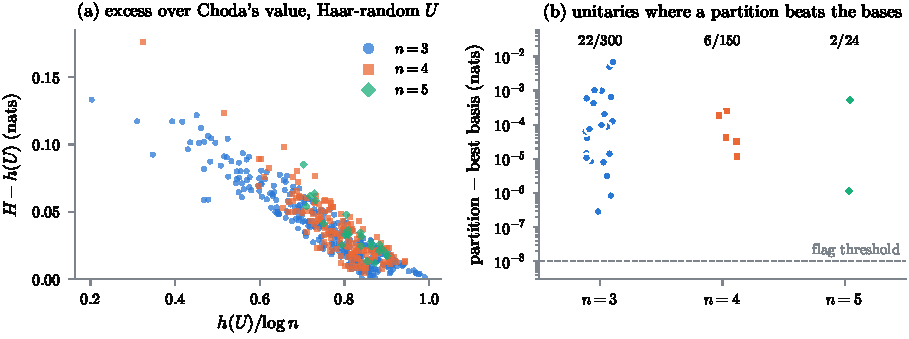
\includegraphics[width=\textwidth]{cs_numerics.pdf}
\caption{Haar-random unitaries, $n=3,4,5$. (a) The excess $H-h(U)$ of the best value found over Choda's value, against the
normalised Choda value $h(U)/\log n$; the excess vanishes as $h(U)\to\log n$ (complementary masas). (b) For the unitaries at
which the best partition found beats the best basis found by more than $\CSFlag$: the difference of the two values, both
recomputed with $\CSDigits$ digits at explicit points; the fractions give the number of such unitaries.}
\label{fig:numerics}
\end{figure}

Table~\ref{tab:cs} and Figure~\ref{fig:numerics} summarise the results; we describe them in order of increasing departure
from the case $n=2$.

\emph{Bases are usually optimal.} For most unitaries the best general partition found is, up to the merging of parallel
elements (Lemma~\ref{lem:F}(a)), an orthonormal basis: the best partition and the best basis agree to $\CSThreeAgree$,
$\CSFourAgree$ and $\CSFiveAgree$ for $n=3,4,5$. For $n=2$ this is Theorem~\ref{thm:n2}.

\emph{But not always.} For $\CSThreeFlagged$ of the $\CSThreeU$ unitaries with $n=3$, $\CSFourFlagged$ of the $\CSFourU$ with
$n=4$ and $\CSFiveFlagged$ of the $\CSFiveU$ with $n=5$, a partition beats the best basis found by more than $\CSFlag$, and none
of these gaps was closed by the extended basis search. The gaps range from $\CSThreeGapMin$ to $\CSThreeGapMax$ for $n=3$, from
$\CSFourGapMin$ to $\CSFourGapMax$ for $n=4$ and from $\CSFiveGapMin$ to $\CSFiveGapMax$ for $n=5$ (Figure~\ref{fig:numerics}(b)).
For the unitary $U'$ with the largest gap the values at the two explicit points are
\[
  \begin{array}{ccc}
  n & \text{partition (a lower bound for }H(\Delta_n|U'\Delta_nU'^*)) & \text{best basis found}\\[2pt]
  3 & \CSThreeGeneral & \CSThreeBasis\\
  4 & \CSFourGeneral & \CSFourBasis\\
  5 & \CSFiveGeneral & \CSFiveBasis
  \end{array}
\]

\emph{The structure of the better partitions.} In all these cases every element of the best partition has rank one, and the
elements point in $\CSThreeDirs$, $\CSFourDirs$ and $\CSFiveDirs$ distinct directions for $n=3,4,5$, that is, in $n+1$ directions;
by Lemma~\ref{lem:F}(a) the partition is, up to the merging tolerance, a partition into $n+1$ rank-one elements. They are
not small perturbations of a basis: two of the directions are far from orthogonal, with the largest overlap
$|\langle d,d'\rangle|$ equal to $\CSThreeOverlap$, $\CSFourOverlap$ and $\CSFiveOverlap$ for the unitaries with the largest gap.

\emph{Choda's partition is never optimal.} In every sample the best value found exceeds $h(U)$, by at least $0.0002$ ($n=3$;
Table~\ref{tab:cs}), as predicted by Proposition~\ref{prop:firstorder} when $M_U$ is not Hermitian. The excess is largest
when $h(U)$ is small and vanishes as $h(U)\to\log n$, in accordance with the characterisation of complementary pairs
(Figure~\ref{fig:numerics}(a)).

\emph{The envelope bound is not attained.} For every sampled unitary the computed $G^*$ exceeds the computed $H$, by at least
$\CSThreeNaiveMin$, $\CSFourNaiveMin$ and $\CSFiveNaiveMin$ for $n=3,4,5$. Unlike for $n=2$, the optimal ensembles do not
appear to consist of maximisers of $G$ (Remark~\ref{rem:envelope}(i)).

\begin{observation}\label{obs:bases}
For $n=3,4,5$ and a small but non-negligible fraction of Haar-random unitaries $U$, the supremum~\eqref{eq:cs} for
$H(\Delta_n|U\Delta_nU^*)$ is not attained at an orthonormal basis: partitions with $n+1$ rank-one elements are better than
every basis found by an extensive multistart search.
\end{observation}

\begin{conjecture}\label{conj:n3}
Let $n\ge3$.
\begin{enumerate}
\item[(a)] There are unitaries $U\in U(n)$ (in fact, a set of positive Haar measure) with
$H(\Delta_n|U\Delta_nU^*)>\max_{W\in U(n)}[h(U^*W)-h(W)]$.
\item[(b)] For Haar-almost every $U$, $h(U)<H(\Delta_n|U\Delta_nU^*)<G^*$.
\end{enumerate}
\end{conjecture}

\subsection{What would make the observations theorems}\label{sec:status}

Conjecture~\ref{conj:n3}(a) would follow from a certified upper bound for the best basis at a single unitary. Indeed, the
value of a fixed partition and the function $B(U)=\max_W[h(U^*W)-h(W)]$ are both continuous in $U$ (the latter as the
maximum of a jointly continuous function over the compact group $U(n)$), so a strict inequality between them at one unitary
persists on a neighbourhood, which has positive Haar measure. Since $h(U^*W)-h(W)$ is invariant under $W\mapsto WD\Pi$ for
diagonal unitaries $D$ and permutation matrices $\Pi$, the maximisation runs over the flag manifold $U(n)/\mathbb{T}^n$, of real
dimension $n(n-1)$, i.e.\ six for $n=3$; for the stored $3\times3$ unitary with the largest gap the margin to be certified is
about $7\times10^{-3}$, which seems within reach of interval branch-and-bound. The lower half of Conjecture~\ref{conj:n3}(b) is
Proposition~\ref{prop:firstorder} together with an almost-everywhere statement for the condition $M_U\ne M_U^*$. For the upper
half, the computed $G^*$ is a certified lower bound for $G^*$, since it is attained at an explicit state, and what is needed
is a certified upper bound for $H$; the dual bound~\eqref{eq:dual} reduces this to exhibiting an affine function $a$ with
$a(\frac1n)<G^*$ and verifying $a\ge G$ on the $(n^2-1)$-dimensional state space, again a single global inequality per
unitary.

\begin{remark}[Non-abelian subalgebras]\label{rem:nonab}
The same computation applies to any pair of subalgebras of $M_n$. For $P=M_2\oplus\C\subset M_3$ and $P=M_2\otimes1\subset M_4$
against $uPu^*$ for two Haar-random $u$ each, the maxima over partitions with $n$, $2n$ and $n^2$ elements agree to
$\CSNonabASpread$ and $\CSNonabBSpread$; we obtain $H=\CSNonabA$ and $H=\CSNonabB$, against $G^*=\CSNonabAG$ and
$G^*=\CSNonabBG$. For $M_2\otimes1\subset M_4$, $E_P\rho=\Tr_2\rho\otimes\frac12$ with the partial trace over the second factor, so
$S(E_P\rho)=S(\Tr_2\rho)+\log2\ge\log2$, and similarly $S(E_Q\rho)\le2\log2$; hence $G^*\le\log2$, a bound that the computed $G^*$
reaches while the computed $H$ stays below it.
\end{remark}

\section{Open problems}\label{sec:open}

\begin{enumerate}
\item[(1)] \emph{A certificate for Observation~\ref{obs:bases}.} Prove Conjecture~\ref{conj:n3}(a) for one explicit unitary,
e.g.\ the stored $3\times3$ unitary with the largest gap, by a rigorous upper bound for $\max_W[h(U^*W)-h(W)]$
(Section~\ref{sec:status}).
\item[(2)] \emph{Explicit formulas for $n\ge3$.} Is there a formula for $H(\Delta_n|U\Delta_nU^*)$ for special families, e.g.\
$U=R_\theta\oplus1_{n-2}$, unitaries close to permutation matrices, or $U$ close to a complementary one? Is $H$ piecewise
analytic in $U$, with the switch between bases and partitions with $n+1$ elements as a transition?
\item[(3)] \emph{Small angles for $n\ge3$.} For $n=2$, $H$ is of first order in the angle $\theta$, while $h(U)$ is of order
$\theta^2\log\frac1\theta$ (Theorem~\ref{thm:bound}). Is $H(\Delta_n|U\Delta_nU^*)$ of first order in the distance of $U$ from the
monomial unitaries for every $n$, and with which constant?
\item[(4)] \emph{The number of elements.} Is the supremum for two masas always attained by a partition with at most $n+1$
elements of rank one? Where partitions beat bases, the best partitions found have rank-one elements in $n+1$ directions,
and otherwise a basis is as good as the best partition found; Proposition~\ref{prop:psw}(b) only guarantees $n^2$ elements.
\item[(5)] \emph{The gap to $G^*$.} Characterise the pairs $P,Q$ with $H(P|Q)=G^*$ (Proposition~\ref{prop:envelope}); for masas,
is equality restricted to $n=2$ and to complementary or commuting pairs?
\item[(6)] \emph{Almost everywhere.} Is $M_U$ non-Hermitian for Haar-almost every $U\in U(n)$, so that
$H(\Delta_n|U\Delta_nU^*)>h(U)$ almost everywhere (Proposition~\ref{prop:firstorder})?
\item[(7)] \emph{Spin model subfactors.} Is the bound of Remark~\ref{rem:bakshi} for $H(R_u|R_v)$ sharp, i.e.\ does
$H(R_u|R_v)=H(\Delta_2|u^*v\Delta_2v^*u)$ hold?
\item[(8)] \emph{Non-abelian subalgebras.} Explicit formulas for the examples of Remark~\ref{rem:nonab}, starting with
$M_2\otimes1\subset M_4$.
\end{enumerate}

\appendix

\section{Numerical method}\label{app:numerics}

All computations for Table~\ref{tab:cs2} (fourth column), Table~\ref{tab:cs}, Figure~\ref{fig:numerics} and
Remark~\ref{rem:nonab} use our PyTorch~\cite{paszke2019} library \texttt{torch\_\allowbreak vn\_\allowbreak algebra}~\cite{lib};
the program is \texttt{scripts/\allowbreak connes\_\allowbreak stormer.py} of the repository~\cite{lib}, run in double precision
(complex128) on a CPU (\CSMode\ run on \CSDevice, \CSSeconds~s in total). The curves of Figures~\ref{fig:bloch}--\ref{fig:asym}
and the third and fifth columns of Table~\ref{tab:cs2} are computed directly from the formulas of Section~\ref{sec:n2} with
NumPy~\cite{harris2020} and SciPy~\cite{virtanen2020} (\texttt{scripts/\allowbreak connes\_\allowbreak stormer\_\allowbreak figures.py}
for the figures).

\paragraph{The functional.} $\Delta_n$ is the image of the inclusion $\C^n\subset M_n$ with inclusion matrix $(1,\dots,1)$,
and $Q_U$ the image of the same inclusion twisted by $U$ (\texttt{inclusions.Inclusion} with \texttt{unitary=U}); the
conditional expectations onto both are taken for the normalised trace $\tau=\Tr/n$, and $\tau\eta(E(x))$ is computed from the
eigenvalues of $E(x)$. The computation is batched and differentiable. The test suite checks it against the plain NumPy
formula~\eqref{eq:Fmasa} to $10^{-12}$ for random partitions with $n=2,3,5$.

\paragraph{Search spaces.} (1) General partitions with $m=n^2$ elements,
\[
  x_j=S^{-1/2}Z_jZ_j^*S^{-1/2},\qquad S=\sum_{j=1}^mZ_jZ_j^*,
\]
with free complex $Z_j\in M_n$; every family with invertible $S$ is a partition of unity, and every partition of unity with
$m$ elements arises this way ($Z_j=x_j^{1/2}$, $S=1$). (2) Orthonormal bases, $x_j=w_jw_j^*$ for the columns $w_j$ of a
unitary $W=W_0\exp(X-X^*)$, with value~\eqref{eq:basis}. (3) States $\rho=ZZ^*/\Tr(ZZ^*)$ for $G^*$; the reported $G^*$ is the
larger of this maximum and the values $G(\rho_j)$ at the normalised elements of the best partition found.

\paragraph{Optimiser.} \texttt{optimize.extremize} runs Adam with the learning rate $0.05\cdot0.6^r$ in rounds $r=0,\dots,7$,
re-centring the unitary chart ($W_0\leftarrow W$, $X\leftarrow0$) after every round, and returns per start the best value
attained at any iterate; every iterate is an admissible point. All starts for all unitaries form one batch. We used
$\CSSteps$ steps for $n=3,4$ and $\CSFiveSteps$ for $n=5$, and the numbers of starts per unitary given in Table~\ref{tab:cs}
($16$ for the states). The unitaries $U$ are Haar-random, from the library's sampler (QR decomposition with phase
correction~\cite{mezzadri2007}), with fixed seeds. For $n=2$ (Table~\ref{tab:cs2}) the search over partitions with four
elements uses $U=D_1R_\theta D_2$ with random phases and $\CSTwoStarts$ starts.

\paragraph{Extended basis search.} A unitary is flagged if the best partition beats the best basis by more than $\CSFlag$. For
every flagged unitary the basis search is repeated with $\CSExtStarts$ further starts, half of them Haar-random and half at
bases built from the directions of the best partition (the principal eigenvectors of its elements, $n$ of them drawn with
probabilities proportional to their traces, perturbed by complex Gaussian noise of size $10^{-3}$ and orthonormalised by the
polar decomposition). For the unitary with the largest remaining gap (for each $n$) another $\CSThreeStressStarts$ starts are
run, again half of each kind.

\paragraph{Recomputation in high precision.} For every unitary that remains flagged, the best partition and the best basis
are recomputed in mpmath with $\CSDigits$ digits: $U$ is replaced by its polar unitarisation $U'=U(U^*U)^{-1/2}$, exactly
unitary at this precision, and the partition $x_j=S^{-1/2}Z_jZ_j^*S^{-1/2}$ is re-normalised from the stored $Z_j$ (for the basis,
$Z_j=w_j$), so that $\|\sum_jx_j-1\|$ is of the order $10^{-50}$. This is a high-precision evaluation, not interval arithmetic.
The flagged unitaries are stored in the file \texttt{connes\_\allowbreak stormer.json} written by the program.

\paragraph{Structure of a partition.} Elements of trace below $10^{-7}$ times the largest trace are discarded; an element counts
as rank one if its second eigenvalue is at most $10^{-6}$ times its trace; the principal eigenvectors $d,d'$ of two elements are
merged into one direction if $|\langle d,d'\rangle|>1-10^{-4}$.

\paragraph{Checks.} For $n=2$ the search over general partitions with four elements reproduces Theorem~\ref{thm:n2} to
$\CSTwoDevLib$, and the optimal basis of Theorem~\ref{thm:n2}(b), evaluated in NumPy, gives the formula to $\CSTwoDevNumpy$
(Table~\ref{tab:cs2}). The test suite \texttt{tests/\allowbreak test\_\allowbreak connes\_\allowbreak stormer.py} checks
$\kappa=1.3254868$ to $10^{-6}$, compares the formula of Theorem~\ref{thm:n2} with a plain BFGS optimisation (SciPy) over
partitions of $M_2$ with three elements for four values of $c$, checks that $300$ random partitions with two to five elements
never exceed it, that the value does not depend on the phases of $U$, the integral representation of $\varphi$ by quadrature,
the Bloch reduction of Lemma~\ref{lem:bloch}, the ensemble identity of Proposition~\ref{prop:psw}(a) for $n=2,3,4$, and the
agreement of the mpmath recomputation with the double-precision value. For complementary masas (Fourier matrices, $n=2,3,4$)
the search gives $H=\log n$ to $\CSFourierDev$ (Remark~\ref{rem:envelope}(ii)), and $H(\Delta_3|\Delta_3)$ vanishes to $\CSSelf$.

\paragraph{Code availability.} The library, the programs that compute all numbers, tables and figures, and the tests are
available at \url{https://github.com/andre-a-no/von_neumann_type_i} (MIT licence).

{\sloppy
\begin{thebibliography}{99}
\bibitem{bakshi} K.~C.~Bakshi, S.~Guin, ``Relative position between a pair of spin model subfactors'', J.\ Aust.\
  Math.\ Soc.\ 119 (2025), no.~1, 1--38; doi:10.1017/S1446788725000035; arXiv:2212.07197.
\bibitem{bengtsson2005} I.~Bengtsson, {\AA}.~Ericsson, M.~Ku\'s, W.~Tadej, K.~\.Zyczkowski, ``Birkhoff's polytope and
  unistochastic matrices, $N=3$ and $N=4$'', Comm.\ Math.\ Phys.\ 259 (2005), 307--324; doi:10.1007/s00220-005-1392-8.
\bibitem{choda} M.~Choda, ``Relative entropy for maximal abelian subalgebras of matrices and the entropy of
  unistochastic matrices'', Internat.\ J.\ Math.\ 19 (2008), 767--776; arXiv:0803.0591.
\bibitem{coles2017} P.~J.~Coles, M.~Berta, M.~Tomamichel, S.~Wehner, ``Entropic uncertainty relations and their
  applications'', Rev.\ Mod.\ Phys.\ 89 (2017), 015002; doi:10.1103/RevModPhys.89.015002.
\bibitem{connes1975} A.~Connes, E.~St{\o}rmer, ``Entropy for automorphisms of II$_1$ von Neumann algebras'', Acta Math.\
  134 (1975), 289--306.
\bibitem{durt2010} T.~Durt, B.-G.~Englert, I.~Bengtsson, K.~\.Zyczkowski, ``On mutually unbiased bases'', Int.\ J.\
  Quantum Inf.\ 8 (2010), 535--640; doi:10.1142/S0219749910006502.
\bibitem{ghosh2026} I.~Ghosh, S.~Kumar, ``Kadison--Kastler distance and interior angle for masas: connections with
  entropy and probabilistic index'', arXiv:2609.38206 (2026).
\bibitem{hall1995} M.~J.~W.~Hall, ``Information exclusion principle for complementary observables'', Phys.\ Rev.\ Lett.\
  74 (1995), 3307--3311; doi:10.1103/PhysRevLett.74.3307.
\bibitem{harris2020} C.~R.~Harris et al., ``Array programming with NumPy'', Nature 585 (2020), 357--362.
\bibitem{jones1983} V.~F.~R.~Jones, ``Index for subfactors'', Invent.\ Math.\ 72 (1983), 1--25.
\bibitem{lib} I.~Nikolaeva, A.~Novikov, ``Finite-dimensional Type I von Neumann algebras in PyTorch: a
  GPU-accelerated framework for random block-diagonal operators'', arXiv:2606.15882 (2026);
  code: \url{https://github.com/andre-a-no/von_neumann_type_i}.
\bibitem{maassen1988} H.~Maassen, J.~B.~M.~Uffink, ``Generalized entropic uncertainty relations'', Phys.\ Rev.\ Lett.\
  60 (1988), 1103--1106; doi:10.1103/PhysRevLett.60.1103.
\bibitem{mezzadri2007} F.~Mezzadri, ``How to generate random matrices from the classical compact
  groups'', Notices Amer.\ Math.\ Soc.\ 54 (2007), 592--604.
\bibitem{neshveyev2006} S.~Neshveyev, E.~St{\o}rmer, \emph{Dynamical Entropy in Operator Algebras}, Ergebnisse der
  Mathematik und ihrer Grenzgebiete (3) 50, Springer, Berlin, 2006; doi:10.1007/3-540-34673-2.
\bibitem{ohya1993} M.~Ohya, D.~Petz, \emph{Quantum Entropy and Its Use}, Texts and Monographs in Physics, Springer,
  Berlin, 1993.
\bibitem{paszke2019} A.~Paszke et al., ``PyTorch: An imperative style, high-performance deep learning
  library'', NeurIPS 2019.
\bibitem{petz2007} D.~Petz, ``Complementarity in quantum systems'', Rep.\ Math.\ Phys.\ 59 (2007), 209--224;
  doi:10.1016/S0034-4877(07)00010-9.
\bibitem{petz2009} D.~Petz, A.~Sz\'ant\'o, M.~Weiner, ``Complementarity and the algebraic structure of 4-level
  quantum systems'', Infin.\ Dimens.\ Anal.\ Quantum Probab.\ Relat.\ Top.\ 12 (2009), 99--116; arXiv:0802.2391.
\bibitem{pimsner1986} M.~Pimsner, S.~Popa, ``Entropy and index for subfactors'', Ann.\ Sci.\ \'Ecole Norm.\ Sup.\ (4)
  19 (1986), 57--106.
\bibitem{popa1983} S.~Popa, ``Orthogonal pairs of $*$-subalgebras in finite von Neumann algebras'', J.\ Operator Theory
  9 (1983), 253--268.
\bibitem{rockafellar1970} R.~T.~Rockafellar, \emph{Convex Analysis}, Princeton Mathematical Series 28, Princeton
  University Press, Princeton, 1970.
\bibitem{tadej2006} W.~Tadej, K.~\.Zyczkowski, ``A concise guide to complex Hadamard matrices'', Open Syst.\ Inf.\
  Dyn.\ 13 (2006), 133--177; arXiv:quant-ph/0512154.
\bibitem{takesaki2002} M.~Takesaki, \emph{Theory of Operator Algebras I}, Springer, 2002.
\bibitem{virtanen2020} P.~Virtanen et al., ``SciPy 1.0: fundamental algorithms for scientific computing in Python'',
  Nat.\ Methods 17 (2020), 261--272.
\bibitem{wootters1989} W.~K.~Wootters, B.~D.~Fields, ``Optimal state-determination by mutually unbiased
  measurements'', Ann.\ Physics 191 (1989), 363--381.
\end{thebibliography}
}

\end{document}
